%!TEX root = thesis.tex

\newcommand{\inp}[1]{\input{../out/#1}}
\newcommand{\characteristic}[2]{\inp{#1/characteristics/#2}}
\newcommand{\descriptive}[2]{\inp{#1/descriptive/#2}}
\newcommand{\test}[3]{\inp{#1/test/#2/#3}}
\newcommand{\normaldistr}{$\mathcal{N}(\descriptive{original}{mean}, \descriptive{original}{variance})$}
\newcommand{\resnormaldistr}{$\mathcal{N}(\descriptive{residual}{mean}, \descriptive{residual}{variance})$}

\newpage

\chapter{Анализ временного ряда в среде R}

В данной главе исследование проводится в программе, рассмотренной в главе 3. Такой подход позволяет быстро и наглядно рассмотреть и проанализировать различные группы данных. При этом инструменты анализа являются гибкими и легко расширяемыми. Что, в свою очередь, позволяет быстро реагировать под особенности определённой задачи.

\section{Детерминированные методы} % (fold)
\label{sec:determenistic}

\subsection{Описательные статистики и первичный анализ данных} % (fold)
\label{sec:basis}

В качестве исследуемых данных примем выборку объема $ n = 38 $ из полученной от учебно-научного центра базы данных, путём отбора наблюдений в июле месяце за период с 1975 по 2012 год. Выборка представлена в приложении \ref{c:source_data} в таблице \ref{table:source}. График исследуемых данных изображён на рисунке \ref{img:input}.
\begin{figure}[ht]
	\center{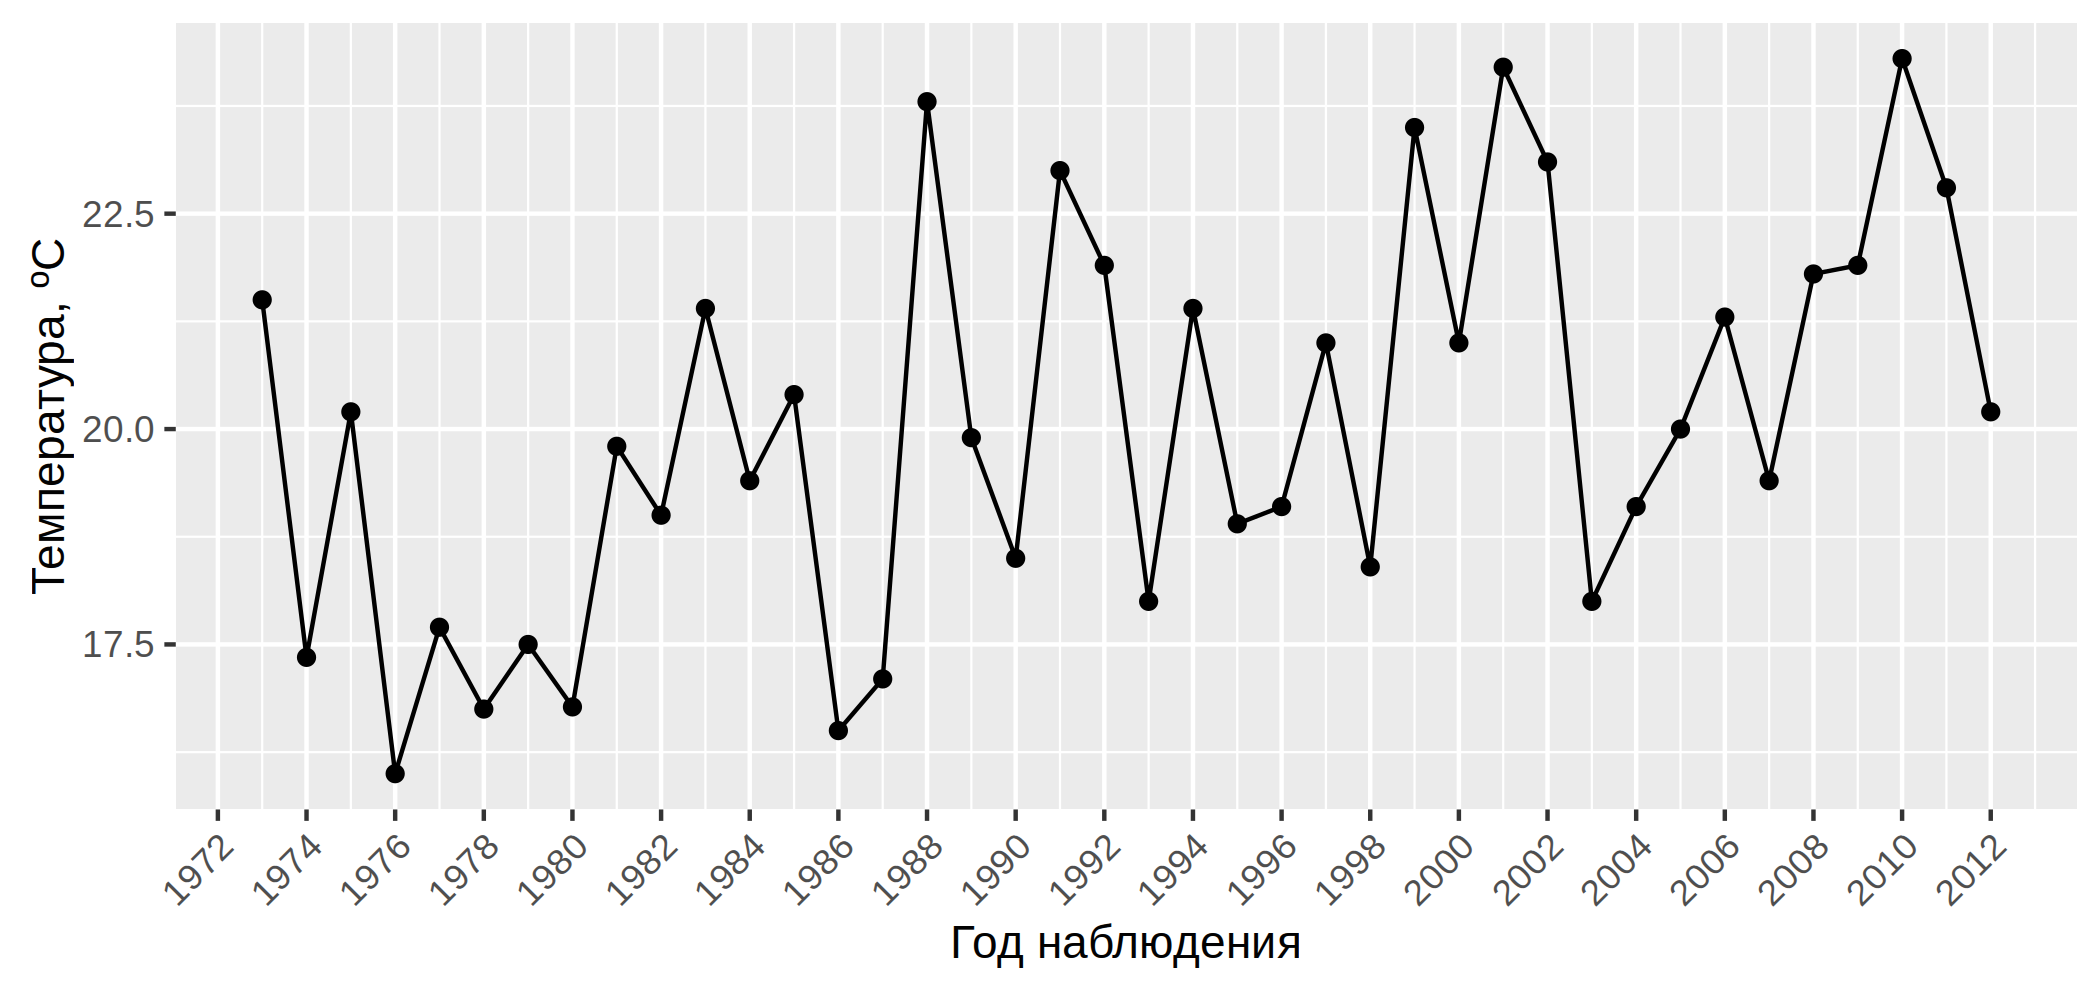
\includegraphics[width=1\linewidth]{../figures/source.png}}
\caption{График исходных данных}
\label{img:input}
\end{figure}

Следует отметить, что для непосредственного изучения в данном разделе были использованы наблюдения с 1975 по 2006 год. Наблюдения за 2007-2012 годы были намеренно исключены из исследования в целях дальнейшего оценивания результатов анализа и прогнозирования. Заметим, что работа, представленная в параграфах \ref{sec:basis}--\ref{sec:regr_analysis}, была также проделана и для всей выборки. Так как поведение целой выборки сохранилось в уменьшенной, то, без потери общности, будем считать её исходной. Обозначим её $ X(t), t = \overline{1, n} $, где $ n $ --- объём выборки, в данном случае равный $ \characteristic{original}{n} $.

Начнём исследование временного ряда с вычисления описательных статистик. Полученные результаты для исходных данных отображены в таблице \ref{table:dstats}.
% latex table generated in R 3.1.2 by xtable 1.7-4 package
% Fri May 15 14:18:49 2015
\begin{table}[ht]
\centering
\begin{tabular}{rr}
  \hline
 & Значение \\ 
  \hline
Среднее & 19.88 \\ 
  Медиана & 19.80 \\ 
  Нижний квартиль & 18.20 \\ 
  Верхний квартиль & 21.40 \\ 
  Минимум & 16.00 \\ 
  Максимум & 24.20 \\ 
  Размах & 8.20 \\ 
  Квартильный размах & 3.20 \\ 
  Дисперсия & 4.92 \\ 
  Стандартное отклонение & 2.22 \\ 
  Коэффициент вариации & 24.75 \\ 
  Стандартная ошибка & 0.37 \\ 
  Асимметрия & 0.18 \\ 
  Ошибка асимметрии & 0.40 \\ 
  Эксцесс & -0.79 \\ 
  Ошибка эксцесса & 0.78 \\ 
   \hline
\end{tabular}
\caption{Описательные статистики для наблюдаемых температур.} 
\label{table:dstats}
\end{table}

Рассмотрим подробнее некоторые полученные статистики.

Как видно из таблицы, \textit{средняя} температура в июле месяце за период с 1975 по 2006 составляет приблизительно 20ºС.

\textit{Коэффициент вариации} в нашем случае равен $ \descriptive{original}{coef-var} $. Из этого следует, что выборку можно считать однородной, так как полученное значение является меньшим 33\% \cite{Eliseeva1995}.

\textit{Коэффициент асимметрии} --- мера симметричности распределения. Полученное значение: $ \descriptive{original}{skew} $. Данное значение говорит о незначительной правосторонней асимметрии распределения. То есть о том, что выборочное распределение можно считать близким к нормальному \cite{Bulmer1979Principles}.

\textit{Коэффициент эксцесса} в рассматриваемом случае равен $ \descriptive{original}{kurtosis}$. Так как коэффициент эксцесса нормального распределения равен $ 0 $, то в данном случае можно говорить о пологости пика распределения выборки по отношению к нормальному распределению \cite{Bulmer1979Principles}.

С помощью тестовых статистик для коэффициента асимметрии и эксцесса \cite[с.85-89]{Cramer1997}, проверим значимость полученных значений для генеральной совокупности. Для этого в модуле \textit{dstats} мной реализованы функции \textit{dstats.test.skew} и \textit{dstats.test.kurtosis}:

Полученная тестовая статистика для коэффициента асимметрии:
\begin{equation*}
	Z_{A_S} = \frac{A_S}{SES} = \descriptive{original}{test-skew}.
\end{equation*}
Данное значение попадает под случай $\vert Z_{A_S} \vert \le 2$, а значит, выборочный коэффициент асимметрии не является значимым. Из чего, в свою очередь, следует, что по нему нельзя судить о коэффициенте асимметрии генеральной совокупности \cite[с.85]{Cramer1997}.

Полученная тестовая статистика для коэффициента эксцесса:
\begin{equation*}
	Z_K = \frac{K}{SEK} = \descriptive{original}{test-kurtosis}.
\end{equation*}
Данное значение попадает под случай $\vert Z_K \vert \le 2$, а значит, в данном случае выборочный коэффициент эксцесса не является значимым и нельзя ничего сказать о коэффициенте эксцесса генеральной совокупности \cite[с.89]{Cramer1997}.

Из полученных результатов следует отметить, что коэффициенты асимметрии и эксцесса, указывают на некоторое отклонение выборочного распределения от нормального закона. Но при этом, из-за небольшого объёма выборки, по этим коэффициентам нельзя судить о соответствующих коэффициентах генеральной совокупности.

С помощью возможностей реализованной программы построим гистограмму для отображения вариационного ряда исходных данных \cite{Chang2012RGraph}. Гистограммы позволяют увидеть, как распределены значения переменных по интервалам группировки, то есть как часто переменные принимают значения из различных интервалов. А также, что бывает более важным, позволяет сделать предположение о виде распределения. Для вычисления интервалов разбиения воспользуемся \textit{формулой Стерджеса}. Из \cite{Sturges1926Choice} количество интервалов разбиения рассчитывается по формуле:
\begin{equation}
\label{eq:sturges}
	k = \lceil log_{2}n \rceil + 1 = \lceil log_{2} \characteristic{original}{n} \rceil + 1 = \characteristic{original}{sturges}.
\end{equation}

Так как по гистограмме можно визуально предположить близость выборочного распределения к нормальному распределению, нанесём на график кривую плотности нормального распределения с параметрами \normaldistr (рисунок \ref{img:histogram_fitted}).
\begin{figure}[ht]
	\center{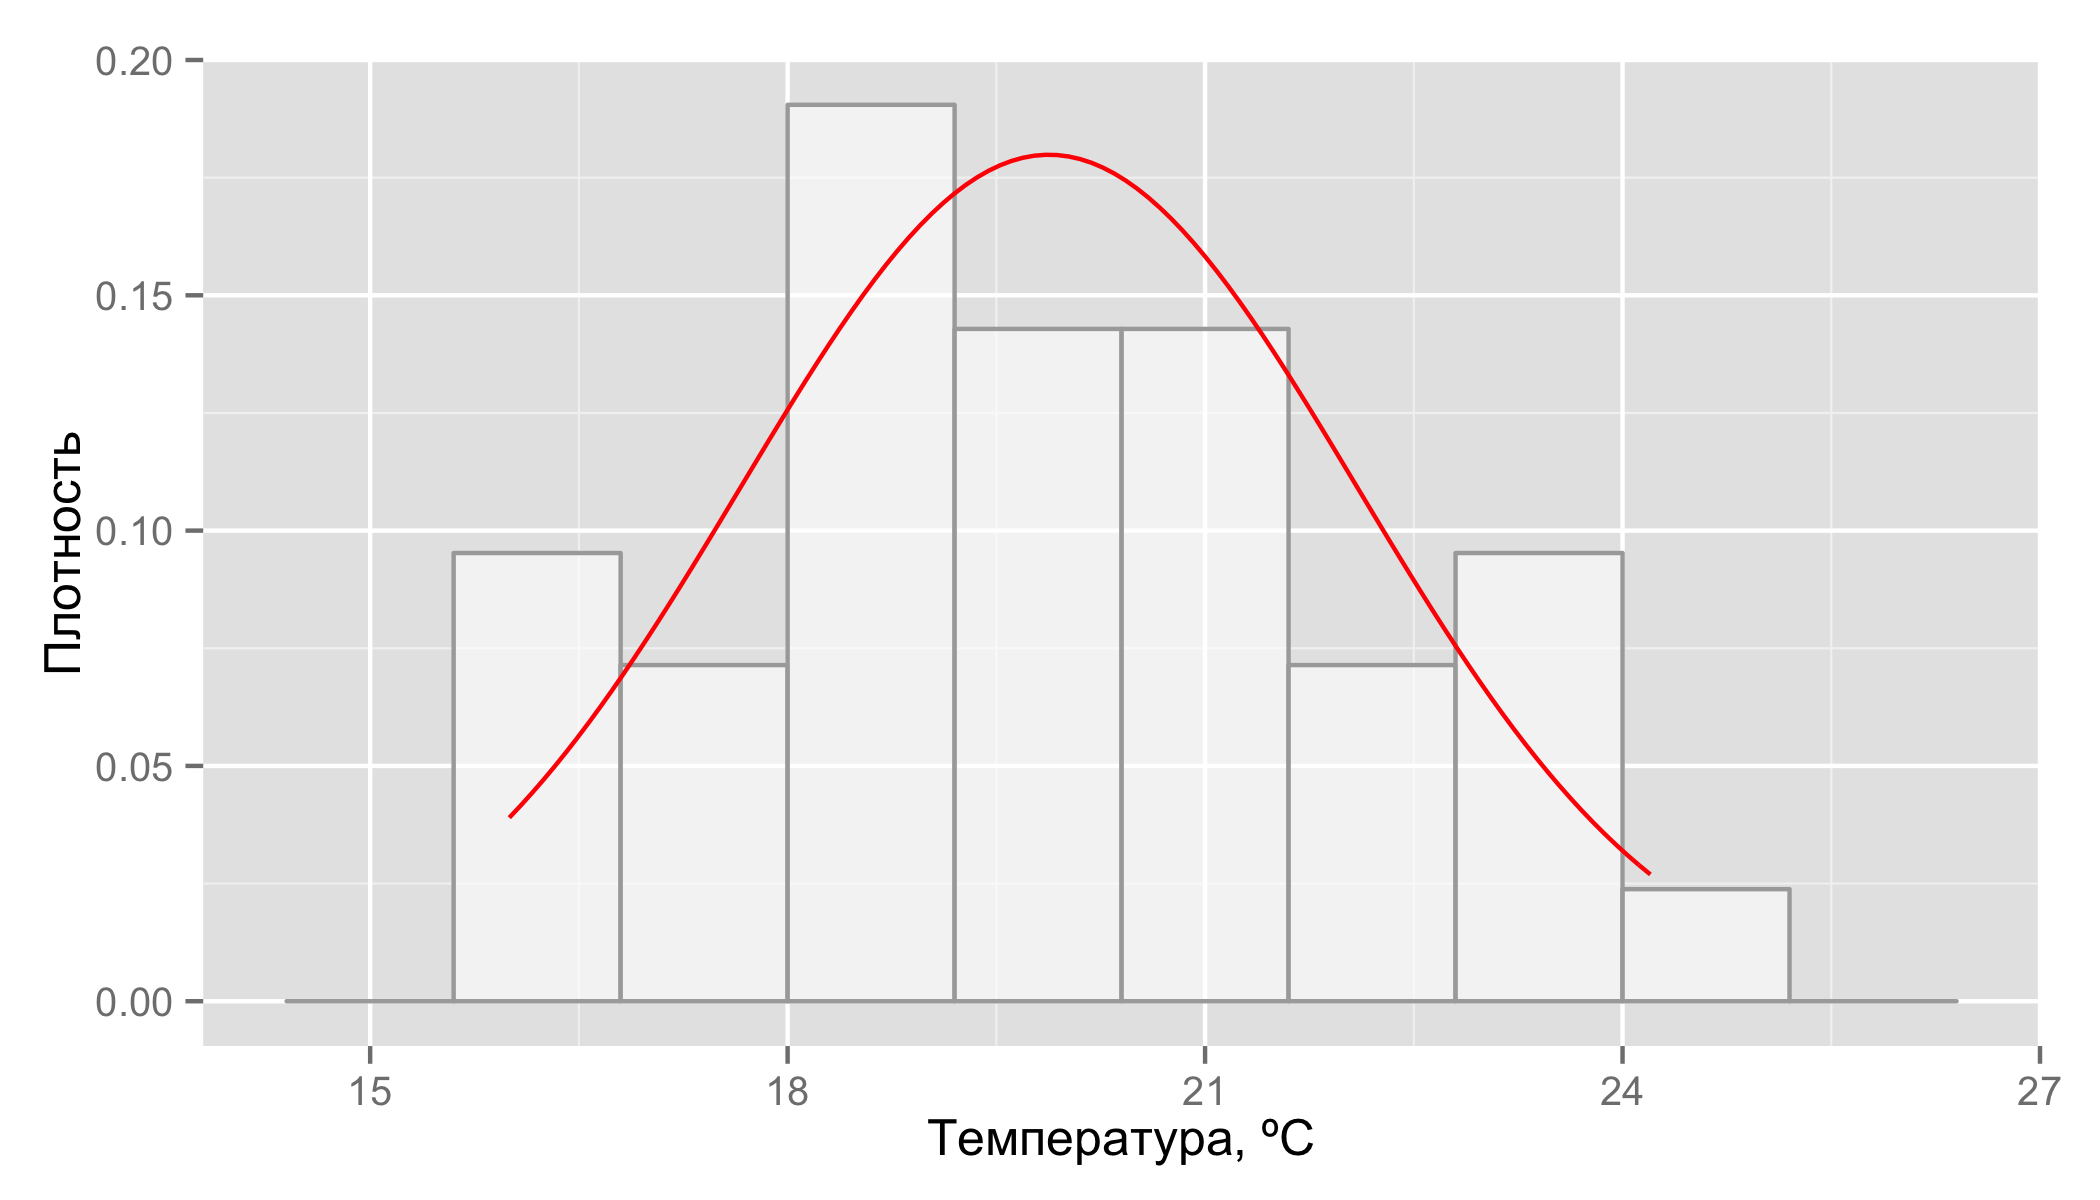
\includegraphics[width=1\linewidth]{../figures/original/histogram.png}}
\caption{Гистограмма наблюдаемых температур с кривой плотности нормального распределения $\mathcal{N}(19.77, 5.12)$}
\label{img:histogram_fitted}
\end{figure}
Проанализируем эту гистограмму. Во-первых, на ней можно заметить небольшую скошенность вправо, что подтверждается показателем асимметрии, полученным на этапе вычисления описательных статистик. Во-вторых, коэффициент эксцесса в описательных статистиках указывал на пологость пика распределения. Данное заключение подтверждается кривой плотности --- она имеет чуть более растянутую колоколообразную форму. Таким образом представленная гистограмма показывает близость выборочного распределения к нормальному с параметрами \normaldistr.

Другим часто используемым графическим способом проверки характера распределения данных является построение т.н. \textit{графиков квантилей}. На таких графиках изображаются квантили двух распределений --- эмпирического (т.е. построенного по анализируемым данным) и теоретически ожидаемого нормального распределения. При нормальном распределении проверяемой переменной точки на графике квантилей должны выстраиваться в прямую линию, исходящую под улом 45 градусов из левого нижнего угла графика. Графики квантилей особенно полезны при работе с небольшими по размеру совокупностями, для которых невозможно построить гистограммы, принимающие какую-либо выраженную форму.

В рамках реализованной программы построен график \ref{img:qqnorm}.
\begin{figure}[ht]
	\center{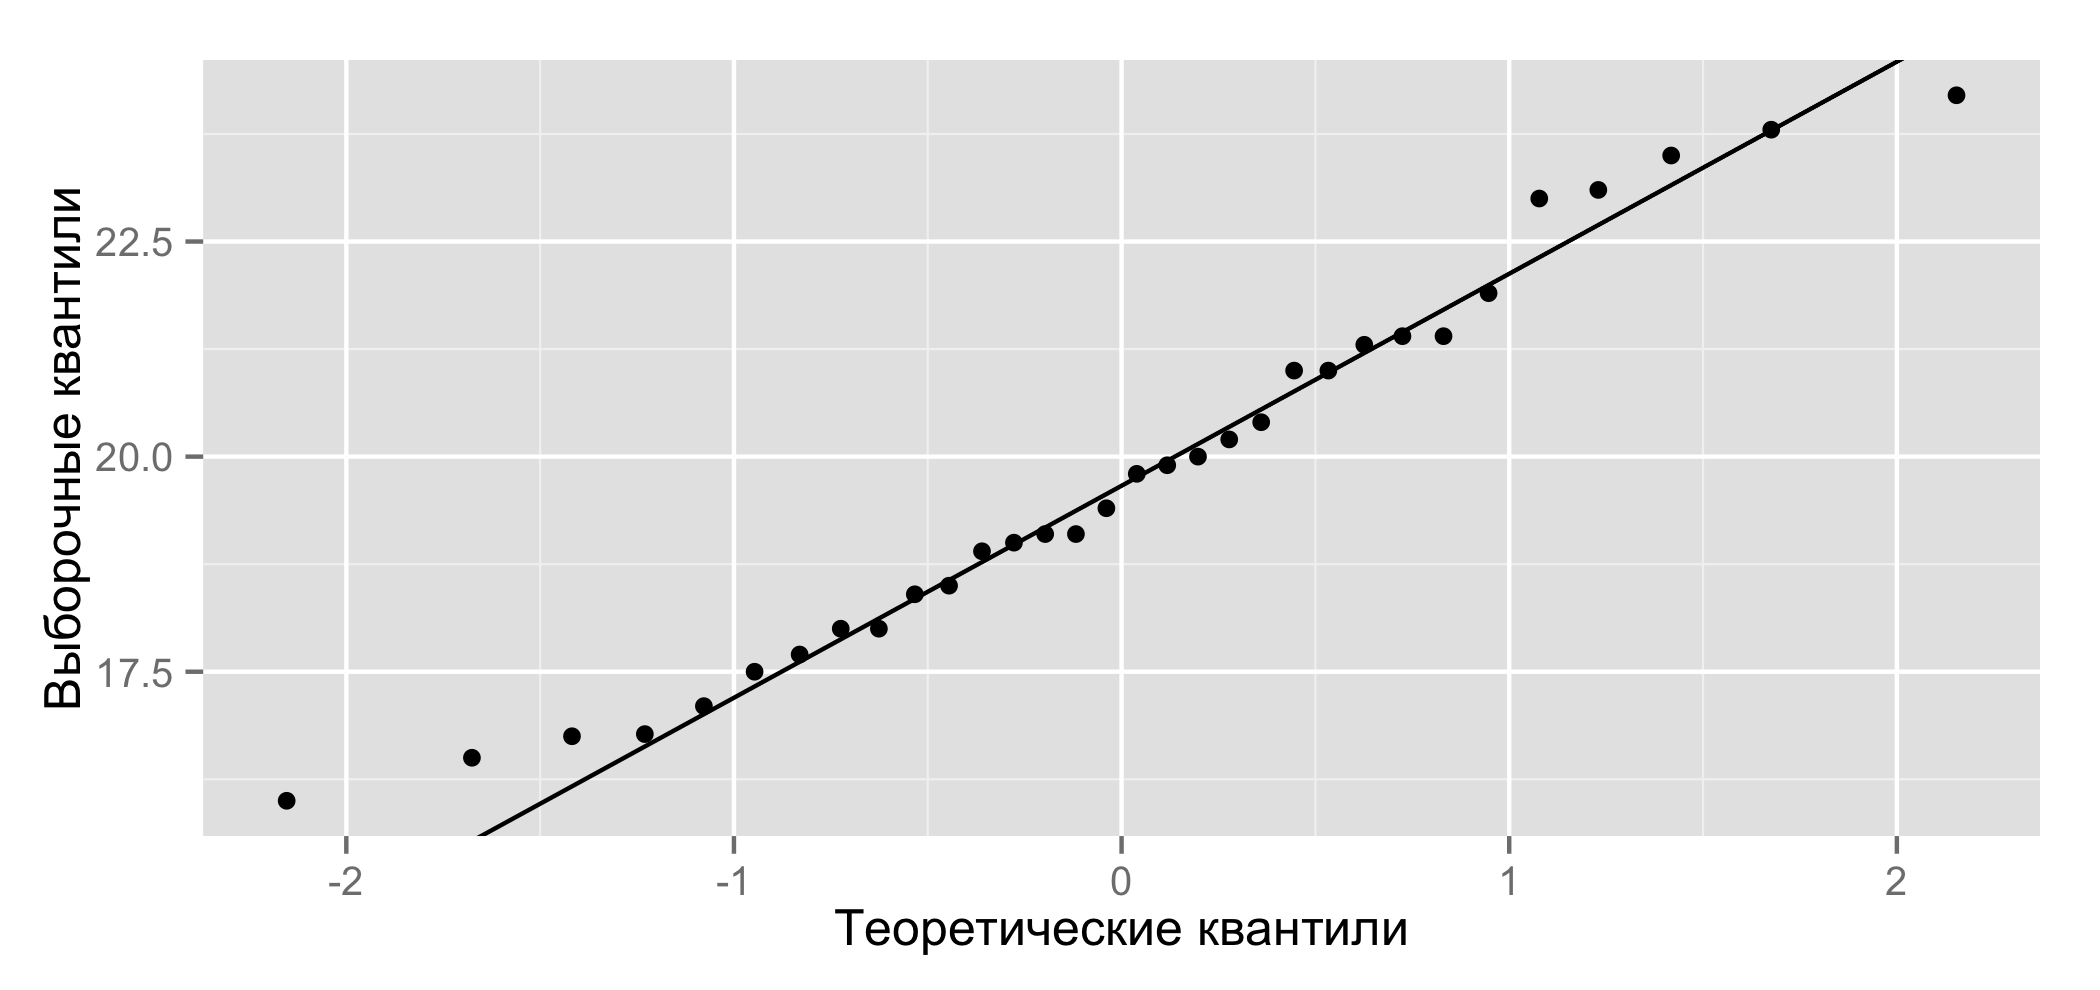
\includegraphics[width=1\linewidth]{../figures/original/quantile.png}}
\caption{График квантилей для наблюдаемых температур}
\label{img:qqnorm}
\end{figure}
На этом графике можно визуально обнаружить нетипичное положение наблюдаемых значений по отношению к нормальному распределению. В данном случае отклонения можно наблюдать на концах рассматриваемого промежутка. Остальные значения образуют отчетливую прямую. Это следует интерпретировать как близость выборочного распределения к нормальному с параметрами \normaldistr.

Далее следует проверить полученные результаты и предположения с помощью некоторых формальных тестов. Существует целый ряд статистических тестов, специально разработанных для проверки нормальности выборочного распределения. В общем виде проверяемую при помощи этих тестов нулевую гипотезу можно сформулировать следующим образом: ``Анализируемая выборка происходит из генеральной совокупности, имеющей нормальное распределение''. Если получаемая при помощи того или иного теста вероятность ошибки $P$ оказывается меньше некоторого заранее принятого уровня значимости (например, $0.05$), нулевая гипотеза отклоняется.

В \textbf{R} реализованы практически все имеющиеся тесты на нормальность --- либо в виде стандарных функций, либо в виде функций, входящих в состав отдельных пакетов. Примером базовой функции является \textit{shapiro.test()}, при помощи которой можно выполнить широко используемый \textit{тест Шапиро-Уилка} \cite{Shapiro1972}. Из полученных в \textbf{R} результатов, статистика Шапиро-Уилка $ W = \test{original}{shapiro}{statistic} $. Вероятность ошибки $ p = \test{original}{shapiro}{p-value} > 0.05 $, а значит нулевая гипотеза не отвергается \cite{Kobzar2006}. Следовательно опровергнуть предположение на основе данного теста нельзя.

Попробуем опровергнуть наше предположение на основе проверки критерия $ \chi^2 $ Пирсона \cite{Gmurman2003}. Для этого воспользуемся пакетом \textit{nortest} и функцией \textit{pearson.test}. Из полученных в \textbf{R} результатов, статистика $\chi^2$ Пирсона $ P = \test{original}{pearson}{statistic}$. Вероятность ошибки $ p = \test{original}{pearson}{p-value} > 0.05 $, а значит нулевая гипотеза не отвергается. Следовательно опровергнуть предположение о нормальности на основе данного теста также нельзя. Проверим критерий: примем уровень значимости $\alpha = 0.05$, тогда из таблицы распределения $\chi^2$ найдём критическое значение критерия $P_{\textrm{кр}}(\alpha, k) = 43.8$. Отсюда следует, что

\begin{equation*}
	P < P_{\textrm{кр}}.
\end{equation*}

А значит, нулевую гипотезу при уровне значимости $\alpha = 0.05$ не отвергаем и подтверждаем сделанный вывод на основании вычисленной вероятности ошибки.

Воспользуемся для тех же целей критерием Колмогорова--Смирнова \cite{Mikulik2002}. Как в предыдущем случае воспользуемся представленной в пакете \textit{nortest} функцией \textit{ks.test}. Из полученных в \textbf{R} результатов, статистика Колмогорова-Смирнова $ D = \test{original}{ks}{statistic}$. Вероятность ошибки $ p = \test{original}{ks}{p-value} > 0.05 $, а значит нулевую гипотезу отвергнуть нельзя. Следовательно опровергнуть предположение о нормальности, как и в предыдущих случаях, также нельзя. Проверим критерий: примем так же уровень значимости $\alpha = 0.05$, тогда критическое значение $D_{\textrm{кр}}(\alpha) = 1.358$. Следовательно,
\begin{equation*}
	D < D_{\textrm{кр}}(\alpha),
\end{equation*}
и подтверждаем сделанные ранее заключения: нельзя отвергнуть нулевую гипотезу о нормальности выборочного распределения.

На данном этапе по полученным ранее результатам возникли подозрения о выбросах в исходной выборке. Выявление таких аномальных значений важно, так как их наличие, как правило, сильно влияет на характеристики выборки, в частности, на коэффициент корреляции. Проверим наличие выбросов с помощью статистических критериев. Для этих целей воспользуемся критерием Граббса \cite{Grubbs1950Sample}. Данный основан на предположении о нормальности исходных данных. То есть, перед применением данного критерия необходимо убедиться, что данные могут быть в разумных пределах аппроксимированы нормальным распределением \cite{grubbs}. Поскольку ранее высказано предположение о нормальности, воспользуемся им для определения наличия выбросов.

Полученные результаты проверки критерия Граббса: статистика $ G = \test{original}{grubbs}{statistic} $, вероятность ошибки $ p\textrm{-value} = \test{original}{grubbs}{p-value} $ --- что однозначно говорит нам о том, что следует отклонить альтернативную гипотезу $H_{1}$ о наличии в выборке выброса. Другими словами, это говорит о том, что в исходной выборке нету выбросов. А значит выборка однородна. Таким образом, подозрения о выбросах не подтвердились проверкой критерия.

В соответствии с результатами проверки критериев и на основе построенных гистограммы и графика квантилей, можно сделать заключение о том, что распределение температуры воды озера Баторино в июле 1975--2009 годов является близким к нормальному закону распределения с параметрами \normaldistr. При этом, обнаружены отклонения от нормальности, описываемые коэффициентами асимметрии и эксцесса. Следует также отметить, что эквивалентные результаты были получены и для всей выборки, до исключения последних наблюдений. При этом, отклонение от нормальности было менее выраженным. Таким образом, отклонение от нормальности можно считать следствием потери информации при исключении наблюдений из исходной выборки.

% subsection basis (end)

\subsection{Корреляционный анализ} % (fold)
\label{sec:corr_analysis}

Исследуем теперь зависимость температуры воды от времени, построив диаграмму рассеяния и вычислив коэффициент корреляции соответствующих переменных.

Диаграммы рассеяния используются для визуального исследования зависимости между двумя переменными. Если переменные сильно связаны, то множество точек данных принимает определённую форму. С помощью таких диаграмм можно наглядно изучить направление зависимости. Если точки на диаграмме расположены хаотически, то это говорит о независимости рассматриваемых переменных. Если с ростом переменной $ t $ возрастает переменная $ X $ то имеет место прямая зависимость. Если же с ростом переменной $ t $ переменная $ X $ убывает, то это указывает на обратную зависимость.
\begin{figure}[ht]
	\center{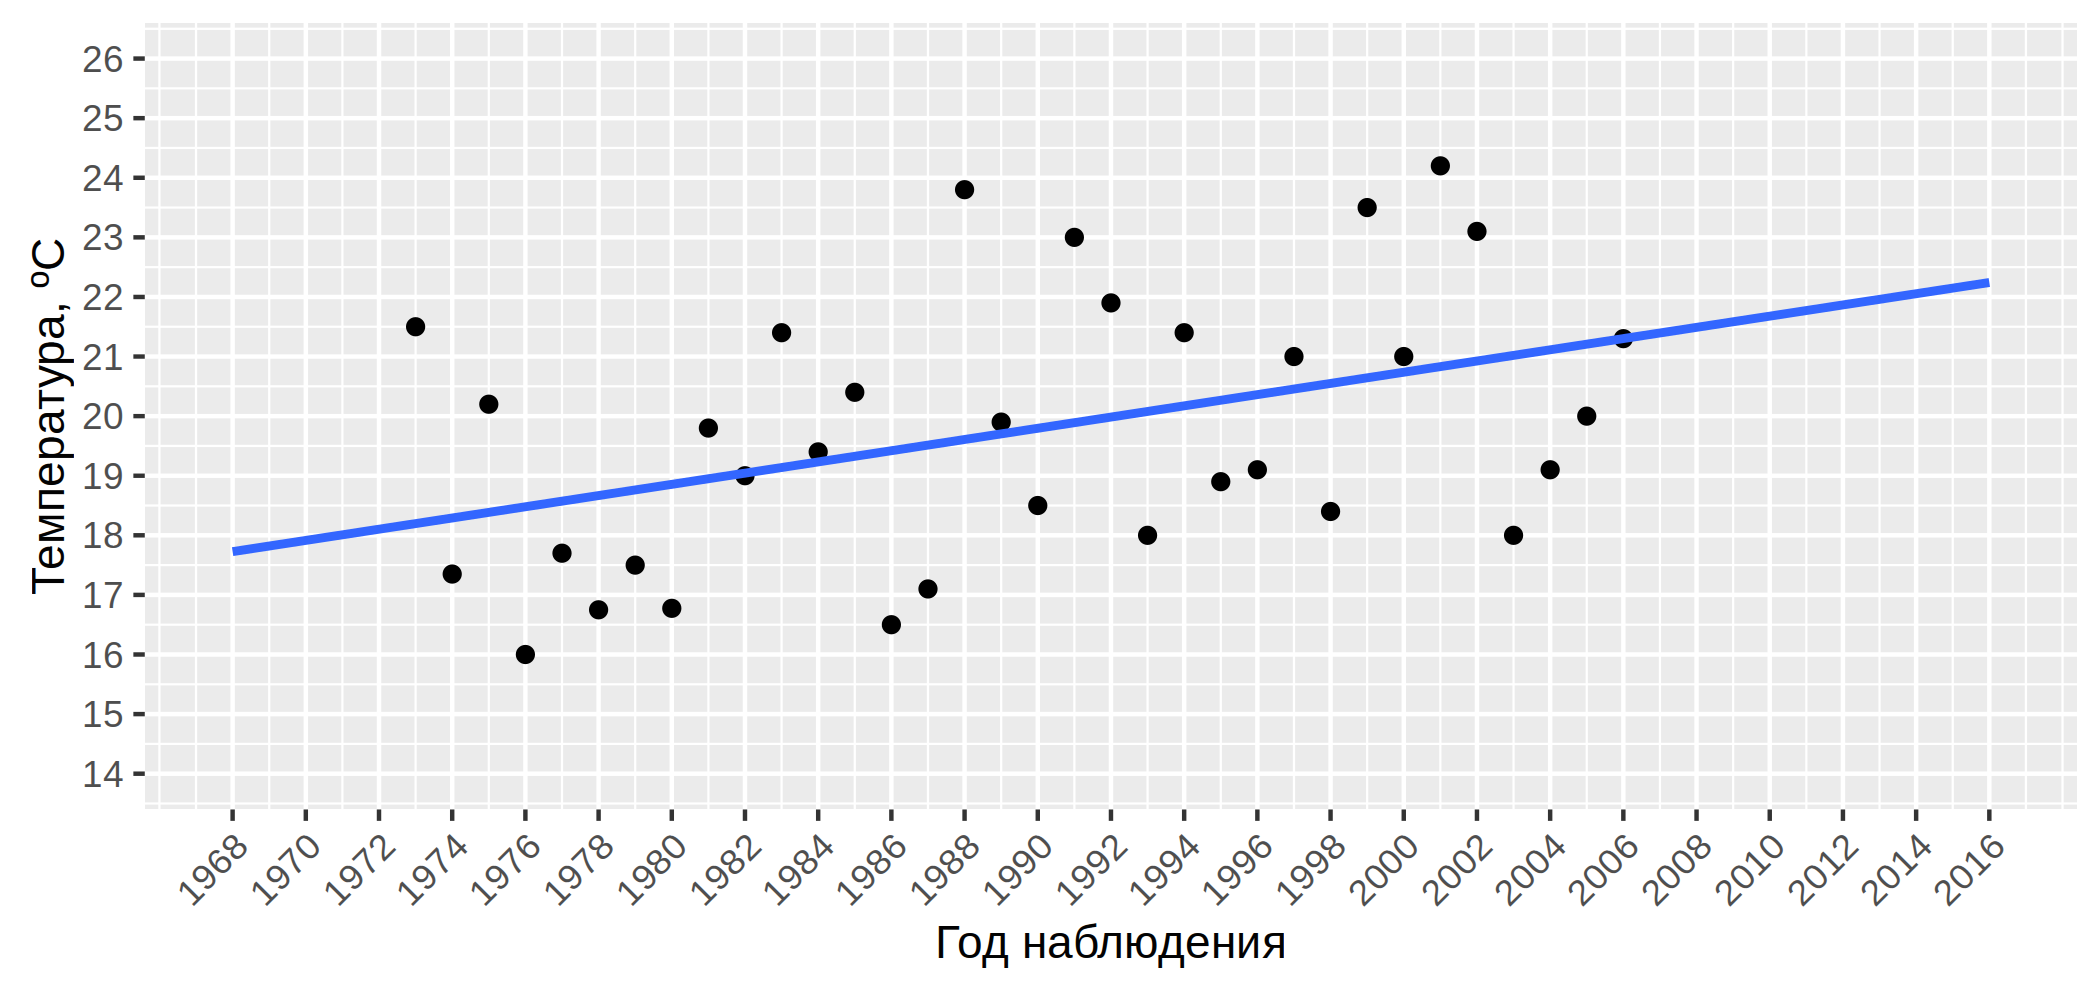
\includegraphics[width=1\linewidth]{../figures/original/scatterplot.png}}
\caption{Диаграмма рассеяния}
\label{img:scatterplot}
\end{figure}

Из рисунка \ref{img:scatterplot} видно, что точки образуют своеобразное <<облако>>, ориентированное вверх, то есть присутствует прямая зависимость между рассматриваемыми переменными. Также, данная диаграмма наглядно показывает силу этой зависимости: так как точки не образуют чёткой формы, а разбросаны относительно линии, то можно говорить о наличии умеренной корреляции.

Проверим полученные результаты подробнее. Из расчётов в \textbf{R}, коэффициент корреляции $ r_{xt} = \characteristic{original}{correlation} $. Этим подтверждаются наши выводы из диаграммы рассеяния о положительной корреляции, поскольку полученный коэффициент корреляции является положительным и присутствует умеренная зависимость: $r_{xt} \approx 0.5$.

Проверим значимость полученного выборочного коэффициента корреляции с помощью критерия Стьюдента:
\begin{equation*}
	T_{\textrm{набл}} = \frac{r_{xt} \sqrt{n - 2}}{\sqrt{1 - r_{xt}^2}} \approx \test{original}{student}{statistic}.
\end{equation*}
Рассмотрим уровень значимости $\alpha = 0.05$. Число степеней свободы $k = n - 2 = \test{original}{correlation}{df}$. Тогда из таблицы критических точек распределения Стьюдента $t_\textrm{кр}(\alpha, k) \approx \test{original}{student}{df}$. Следовательно,
\begin{equation*}
	T_{\textrm{набл}} > t_\textrm{кр}(\alpha, k).
\end{equation*}
Значит нулевую гипотезу о равенстве нулю коэффициента корреляции генеральной совокупности следует отклонить \cite{Eliseeva1995}.

Также оценим значимость с помощью возможностей пакета \textbf{R} и функции \textit{cor.test}. Представленная функция позволяет с помощью различных методов выполнять проверки значимости выборочного коэффициента корреляции. Воспользуемся проверкой теста методом Пирсона. Из результатов её выполнения статистика $ t = \test{original}{correlation}{statistic} $, количество степеней свободы $ df = \test{original}{correlation}{df} $ и вероятность ошибки $p = \test{original}{correlation}{p-value} < 0.05$, следовательно это говорит о том, что необходимо отвергнуть гипотезу о равенстве нулю коэффициента корреляции генеральной совокупности.

Результаты обоих подходов в проверке значимости совпали. Другими словами, выборочный коэффициент значимо отличается от нуля, т.е. температура воды и время при уровне значимости $\alpha = 0.05$ имеют прямую умеренную зависимость.

Следовательно, в рассматриваемом случае можно говорить о присутствии значимой корреляции между температурой воды в озере Баторино и временем. Что говорит росте температуры окружающей среды с момента начала наблюдений.

% subsection corr_analysis (end)

\subsection{Регрессионный анализ} % (fold)
\label{sec:regr_analysis}

Для введения последующих понятий анализа временных рядов воспользуемся \cite{Eddows1997}.

Во временных рядах выделяют три составляющие:
\begin{enumerate}
	\item \textit{Тренд (тенденция развития) $ y $} --- эволюционная составляющая, которая характеризует общее направление развития изучаемого явления и связанна с действием долговременных факторов развития.
	\item \textit{Циклические $ k $, сезонные колебания $ s $} --- это составляющие, которые проявляются как отклонения от основной тенденции развития изучаемого явления, и связанны с действие краткосрочных, систематических факторов развития.
	\item \textit{Нерегулярная случайная составляющая (ошибка) $ \varepsilon $}, являющаяся результатом действия второстепенных факторов развития.
\end{enumerate}
Первые два типа компонент представляют собой детерминированные составляющие. Случайная составляющая образована в результате суперпозиции некоторого числа внешних факторов.

По типу взаимосвязи вышеперечисленных составляющих ряда динамики можно построить следующие модели временных рядов:
\begin{itemize}
	\item Аддитивная модель: $ x = y + k + s + \varepsilon $;
	\item Мультипликативная модель: $x = y \times k \times s \times \varepsilon$.
\end{itemize}

Аддитивной модели свойственно то, что характер циклических и сезонных колебаний остаётся постоянным. В мультипликативной модели характер циклических и сезонных колебаний остаётся постоянным только по отношению к тренду (т.е. значения этих составляющих увеличиваются с возрастанием значений тренда).

По причине того, что в данном случае мы рассматриваем среднюю температуру июля месяца каждого года на протяжении длительного периода, будем считать, что в рассматриваемом временном ряде циклическая и сезонная составляющие отсутствуют.

При проведении корреляционного анализа, на графике \ref{img:scatterplot} был замечен явно выраженный линейный рост значений со временем. Что впоследствии было подтверждено критериями. Из этого следует, что уравнение тренда имеет вид:
\begin{equation*}
	y(t) = at + b,
\end{equation*}
где $ a, b \in \mathbb{R} $ -- коэффициенты модели, $ t = \overline{1, n} $, $ n $ --- объем выборки.

Продолжая рассуждение, как наблюдение из графика, можно отметить, что не происходит увеличения амплитуды колебаний с течением времени. А значит, искомая модель является аддитивной. Из всего вышесказанного можно заключить, что модель исходного временного ряда имеет вид:
\begin{equation*}
	x = y + \varepsilon,
\end{equation*}
где $ y $ -- тренд, $ \varepsilon $ - нерегулярная составляющая.

В \textbf{R} реализованы функции, позволяющие подгонять линейные модели к исследуемым данным \cite{Shumway2006Time}. Одной из таких функций является \textit{lm(Fitting Linear Model)} \cite[c.178]{Kabacoff2009R}. Она позволяет получить коэффициенты линии регрессии. Таким образом, можно вычислить одну из искомых компонент -- тренд. И как следствие, после его удаления из исходных данных, получим нерегулярную составляющую $ \varepsilon(t) $. Коэффициенты, полученные с помощью данной функции представлены в \eqref{eq:regr_coeff}.
\begin{equation}
\label{eq:regr_coeff}
	a = \characteristic{original}{sign-a}, \quad b = \characteristic{original}{sign-b}.
\end{equation}
Следует отметить, что в пакете \textbf{STATISTICA} похожая процедура была проведена для всей выборки с помощью инструмента \textit{Trend Subtract}, результаты которой совпадают с полученными коэффициентами в \textbf{R}.

Таким образом получена линейная модель, описывающая тенденцию развития:
\begin{equation}
\label{eq:regr}
	y(t) = at + b = \characteristic{original}{sign-a}t + \characteristic{original}{sign-b}
\end{equation}

На основе полученной линейной модели \eqref{eq:regr}, построим ряд остатков, удалив тренд из исходного ряда. Полученный ряд представлен в приложении \ref{c:app_results} в таблице \ref{table:residuals} и графически на рисунке \ref{img:ts_detrended}.
\begin{figure}[ht]
	\center{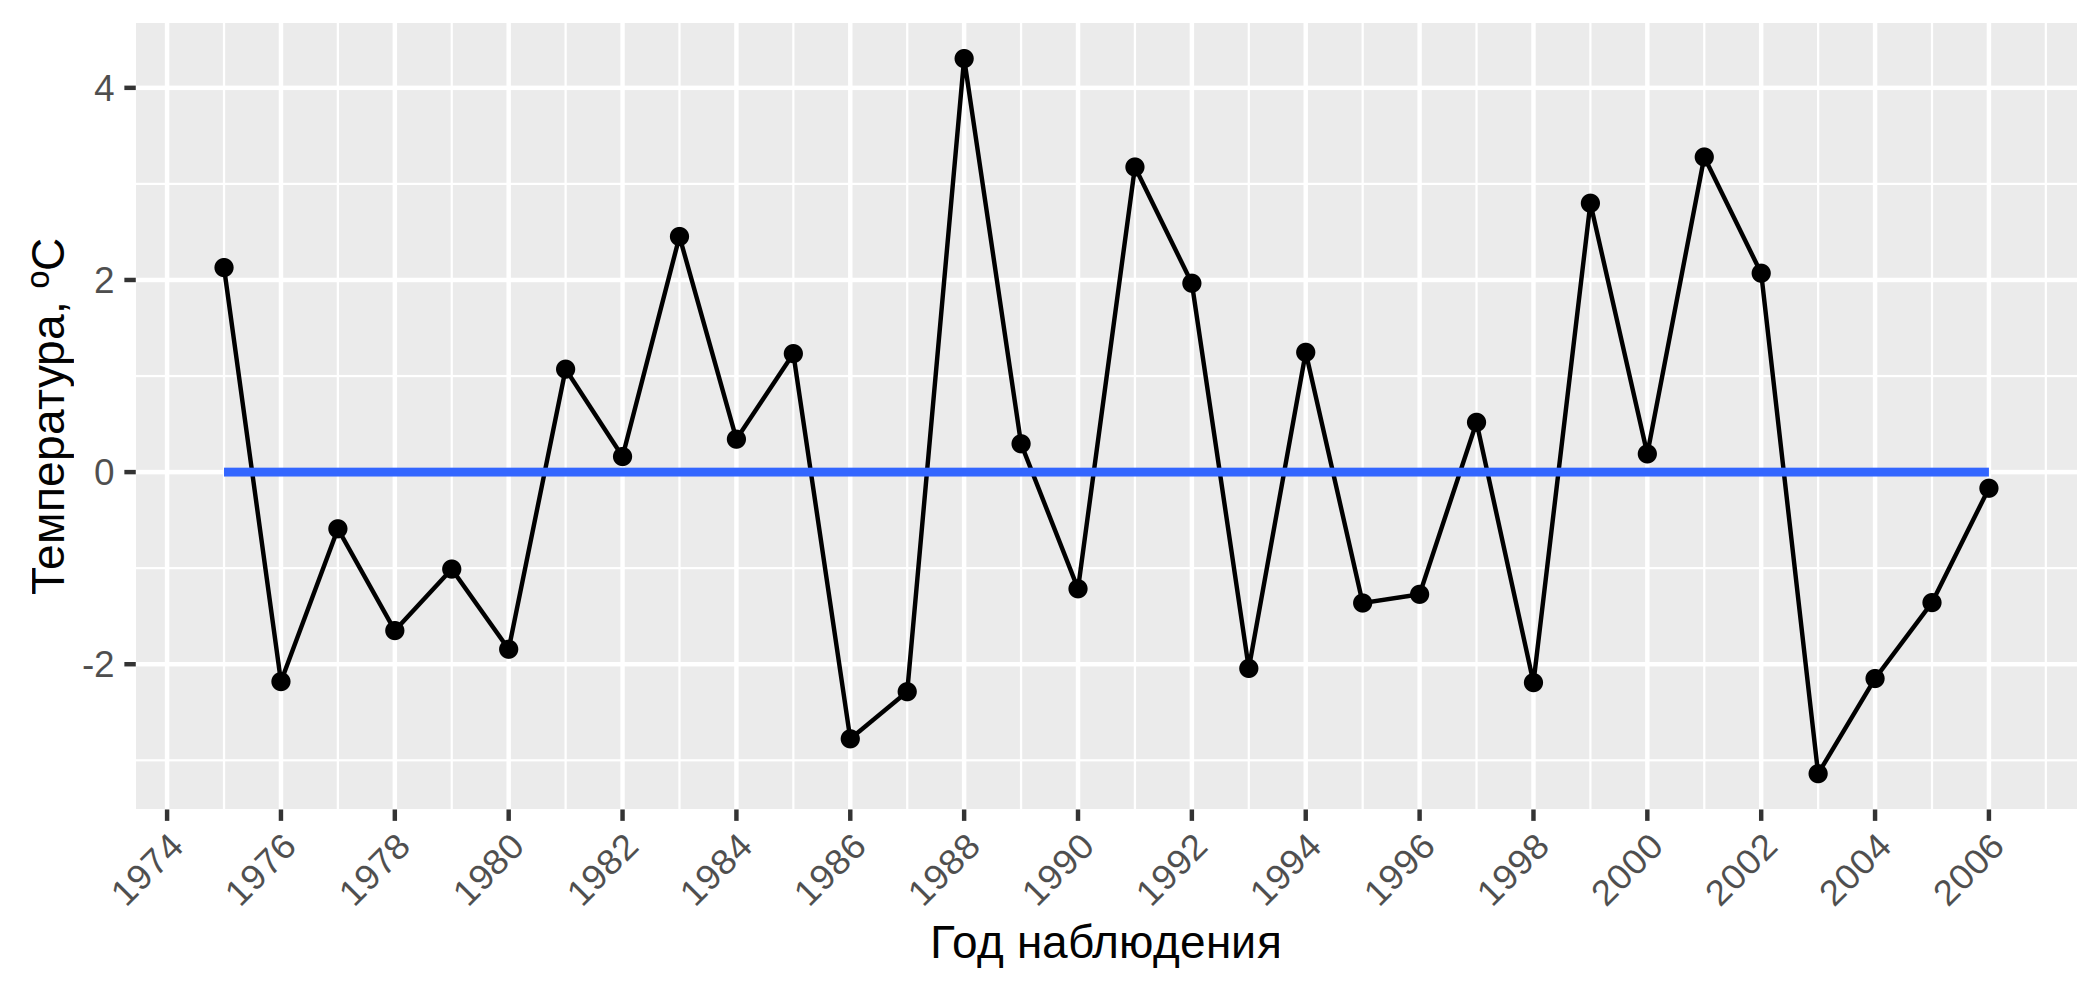
\includegraphics[width=1\linewidth]{../figures/residual/time-series.png}}
\caption{Нерегулярная составляющая $ \varepsilon(t) $}
\label{img:ts_detrended}
\end{figure}

Проведём анализ полученной регрессионной модели. Для этого проверим значимость полученных коэффициентов регрессии и оценим адекватность построенной регрессионной модели.

Рассчитаем вспомогательные величины, воспользовавшись \cite{Eddows1997}. Дисперсия отклонения
\begin{equation*}
	\sigma_{\varepsilon}^2 \approx \characteristic{original}{sign-vardev},
\end{equation*}
стандартные случайные погрешности параметров $a, b$:
\begin{equation*}
	\sigma_{a} \approx \characteristic{original}{sign-errorA}, \quad \sigma_{b} \approx \characteristic{original}{sign-errorB}.
\end{equation*}

Воспользуемся критерием значимости коэффициентов линейной регрессии \cite{Eliseeva1995}. Примем уровень значимости $\alpha = 0.05$, тогда
\begin{equation*}
	T_{a} = \characteristic{original}{sign-studentA}, \quad T_{b} = \characteristic{original}{sign-studentB}.
\end{equation*}

Число степеней свободы $k = \characteristic{original}{sign-df}$, $t_{\textrm{кр}}(k, \alpha) = \characteristic{original}{sign-critical}$.

\begin{itemize}
	\item $\vert T_{a} \vert > t_{\textrm{кр}}$ $\Rightarrow$ коэффициент $a$ значим.
	\item $\vert T_{b} \vert > t_{\textrm{кр}}$ $\Rightarrow$ коэффициент $b$ значим.
\end{itemize}
Следовательно, при уровне значимости $\alpha = 0.05$, коэффициенты линейной регрессии являются значимыми.

Оценим адекватность полученной регрессионной модели. Дисперсия модели:
\begin{equation*}
	\overline{\sigma^2} \approx \characteristic{original}{adeq-var_}.
\end{equation*}

Остаточная дисперсия:
\begin{equation*}
	\overline{D} \approx \characteristic{original}{adeq-resvar}.
\end{equation*}

Воспользуемся F-критерием Фишера. Пусть уровень значимости $\alpha = 0.05$,
\begin{equation*}
	F_{\textrm{крит}} \approx \characteristic{original}{adeq-statistic},
\end{equation*}
при степенях свободы $v_1 = 1, v_2 = \characteristic{original}{sign-df}, F_{\textrm{табл}}(v_1, v_2, \alpha) = \characteristic{original}{adeq-critical}$.

\begin{equation*}
	F_{\textrm{крит}} > F_{\textrm{табл}}.
\end{equation*}
Следовательно, при уровне значимости $\alpha = 0.05$, регрессионная модель является адекватной.

Рассчитаем коэффициент детерминации:
\begin{equation*}
	\eta_{x(t)}^2 \approx \characteristic{original}{adeq-determination}.
\end{equation*}

Проверим отклонение от линейности: $\eta_{x(t)}^2 - r_{xt}^{2} \approx \characteristic{original}{adeq-linearity} \le 0.1$. Следовательно отклонение от линейности незначительно. Но при этом коэффициент детерминации оказался не высоким($<0.7$), это говорит о том, что построенная регрессионная модель не описывает в достаточной мере поведение временного ряда. Это, в свою очередь, может значить, что изменение температуры зависит не только от времени, но ещё и от каких-то других, неучтённых, факторов.

Тем не менее, построим прогноз по полученной модели. Вычисленные прогнозные значения на 2007-2012 годы для сравнения отображены в таблице \ref{table:prediction_trend}:
% latex table generated in R 3.1.3 by xtable 1.7-4 package
% Thu May 21 14:09:02 2015
\begin{table}[ht]
\centering
\begin{tabular}{rrrr}
  \hline
 & Год & Актуальное & Прогнозное \\ 
  \hline
1 & 2007 & 19.40 & 18.07 \\ 
  2 & 2008 & 21.80 & 18.18 \\ 
  3 & 2009 & 21.90 & 18.29 \\ 
  4 & 2010 & 24.30 & 18.40 \\ 
  5 & 2011 & 22.80 & 18.51 \\ 
  6 & 2012 & 20.20 & 18.62 \\ 
   \hline
\end{tabular}
\caption{Сравнение прогнозных значений (тренда)} 
\label{table:prediction_trend}
\end{table}

% TODO добавить возможно MSE
Имеющееся отклонение прогнозов от реальных данных ещё раз подтверждает, что построенная модель временного ряда обладает невысокой точностью. И поэтому необходимо её улучшать другими методами.

% TODO Окончательно сказать, что тут использовалась СТАСТИСТИКА или где-нибудь в заключении

% subsection regr_analysis (end)

\subsection{Анализ остатков} % (fold)
\label{sub:analysis_residuals}

Проанализируем полученную на этапе регрессионного анализа нерегулярную составляющая $ \varepsilon(t) $. Для этого проверим свойства, которым она должна удовлетворять:
\begin{enumerate}
	\item Математическое ожидание $ \varepsilon(t) $ равно $ 0 $;
	\item Дисперсия $ \varepsilon(t) $ постоянна для всех значений;
	\item Остатки независимы и нормально распределены.
\end{enumerate}
Вычислим описательные статистики для остатков. Полученные результаты проследим по таблице \ref{table:residuals_dstats}.
% latex table generated in R 3.1.2 by xtable 1.7-4 package
% Mon Mar  2 02:32:46 2015
\begin{table}[ht]
\centering
\begin{tabular}{rr}
  \hline
 & Значение \\ 
  \hline
Среднее & -0.00 \\ 
  Медиана & 0.14 \\ 
  Нижний квартиль & -1.80 \\ 
  Верхний квартиль & 1.28 \\ 
  Минимум & -2.99 \\ 
  Максимум & 4.33 \\ 
  Размах & 7.32 \\ 
  Квартильный размах & 3.07 \\ 
  Дисперсия & 3.84 \\ 
  Стандартное отклонение & 1.96 \\ 
  Коэффициент вариации & 0.00 \\ 
  Стандартная ошибка & 0.33 \\ 
  Асимметрия & 0.42 \\ 
  Ошибка асимметрии & 0.40 \\ 
  Эксцесс & -0.77 \\ 
  Ошибка эксцесса & 0.78 \\ 
   \hline
\end{tabular}
\caption{Описательные статистики остатков} 
\label{table:residuals_dstats}
\end{table}


Как видно из таблицы \ref{table:residuals_dstats}, среднее значение равно нулю. При этом коэффициенты асимметрии($ A_S = \descriptive{residual}{skew} $) и эксцесса($ K = \descriptive{residual}{kurtosis} $) указывают на большее отклонение распределения остатков от нормального закона по сравнению с исходным случаем.

Построим гистограмму и график квантилей для проверки последних заключений. Построенная гистограмма (приложение \ref{c:graphs}, рисунок \ref{img:resid_hist}) демонстрирует скошенность вправо и пологость пика, отображённой кривой нормального распределения. Данные наблюдения согласуются с полученными в таблице \ref{table:residuals_dstats} коэффициентами асимметрии и эксцесса.
\begin{figure}[ht]
	\center{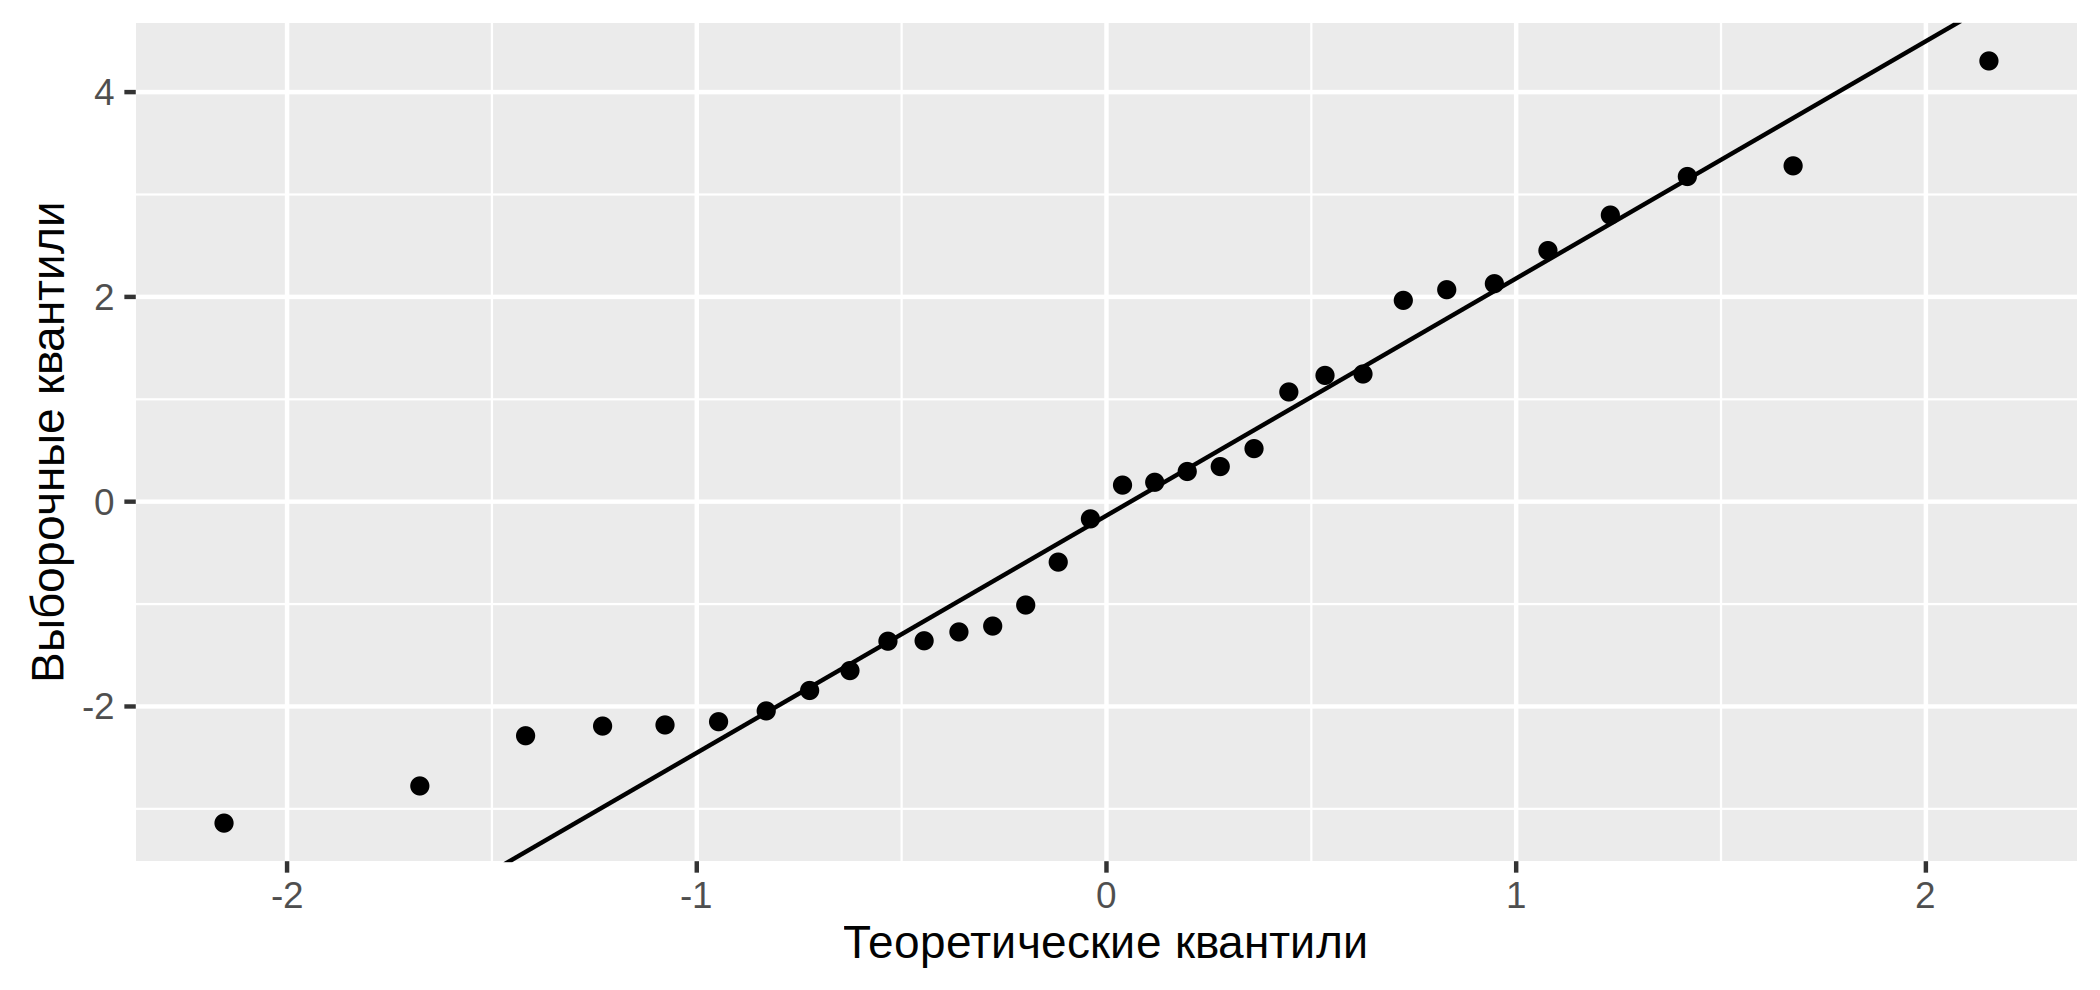
\includegraphics[width=1\linewidth]{../figures/residual/quantile.png}}
\caption{График квантилей для остатков}
\label{img:resid_qqnorm}
\end{figure}

На рисунке \ref{img:resid_qqnorm} можно заметить, что присутствуют отклонения относительно нормального распределения. Наиболее явный из них --- нижний хвост. Остальные --- небольшие скачки по ходу линии нормального распределения. Проверим с помощью критерия Шапиро-Уилка, можно ли считать полученные остатки нормально распределёнными. Из полученных в \textbf{R} результатов, статистика Шапиро--Уилка $ W = \test{residual}{shapiro}{statistic} $. Вероятность ошибки $ p = \test{residual}{shapiro}{p-value} > 0.05 $, а значит нулевая гипотеза, сформулированная ранее, не отвергается. Следовательно опровергнуть предположение о нормальности на основе данного теста нельзя.

Проверим критерий $ \chi^2 $ Пирсона. Из полученных в \textbf{R} результатов, статистика $\chi^2$ Пирсона $ P = \test{residual}{pearson}{statistic}$. Вероятность ошибки $ p = \test{residual}{pearson}{p-value} > 0.05 $, а значит нулевая гипотеза не отвергается.

Построим график автокорреляционной функции для определения наличия взаимосвязей в ряде остатков (рисунок \ref{img:resid_acf}). На графике пунктирные линии разграничивают значимые и не значимые корреляции: значения, выходящие за линии, являются значимыми \cite[с.376]{Teetor2011RCook}. На представленном графике автокорреляционной функции все значения не выходят за интервал, обозначенный пунктирными линиями. Это означает, что в представленной автокорреляционной функции нету значимых автокорреляций. Проверим это замечание с помощью теста Льюнга-Бокса \cite[с.377-378]{Teetor2011RCook}. Данный тест позволяет проверить наличие автокорреляций в исследуемых данных. Используя возможности пакета \textbf{R} получили значения: статистика Льюнга--Бокса $ X^2 = \test{residual}{ljung-box}{statistic} $ и вероятность ошибки $ p = \test{residual}{ljung-box}{p-value} > 0.05$ --- это говорит о том, что тест не выявил значимых автокорреляций.

\begin{figure}[ht]
	\center{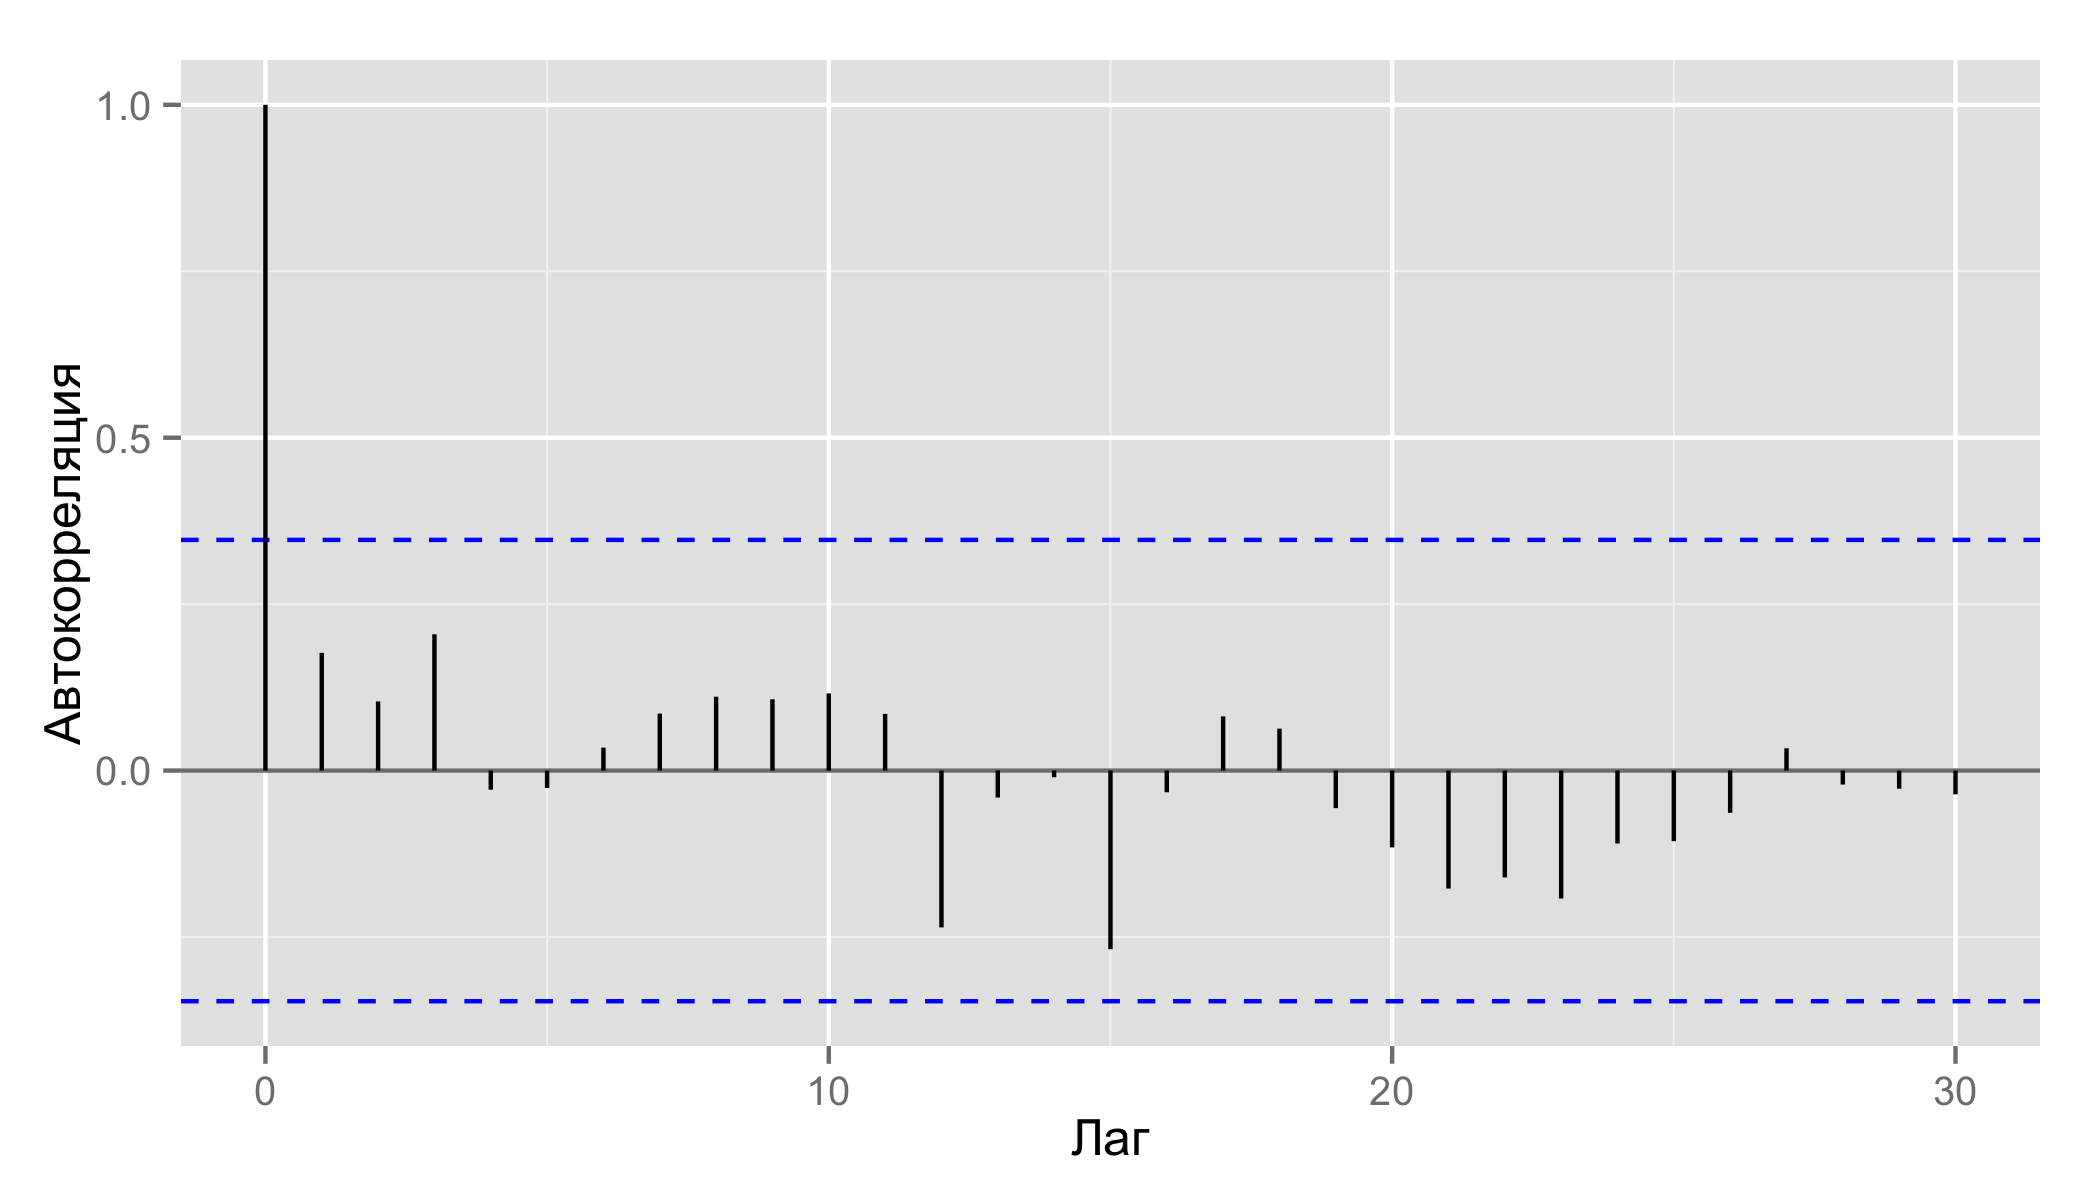
\includegraphics[width=1\linewidth]{../figures/residual/acf.png}}
\caption{График автокорреляционной функции}
\label{img:resid_acf}
\end{figure}

На рисунке \ref{img:resid_acf} также можно заметить резкое затухание значений автокорреляций с увеличением лага. На основе этого можно сделать предположение о стационарности в широком смысле. Для проверки этого предположения воспользуемся расширенным тестом Дики--Фуллера(ADF) \cite{Dickey1979Distribution}. Из результатов проверки теста, статистика Дики-Фуллера $ DF = \test{residual}{stationarity}{statistic} $, вероятность ошибки $ p = 0.04 < 0.05 $. Следовательно, при уровне значимости $ \alpha = 0.05 $ необходимо принять альтернативную гипотезу о стационарности.
% TODO: надо подумать. p-value для обрезанного ряда оказался не вери-гуд // ПОДОГНАТЬ

% TODO: нужно проапдейтить вывод -- он плохой // проапдейтил // независимые ~ нет автокорелляций
Таким образом в результате анализа детерминированными методами выделены две составляющие исходной модели данных: тренд и нерегулярная составляющая. В ходе регрессионного анализа было показано, что модель, основанная на тренде, не позволяет воспроизвести поведение исходного временного ряда. То есть нерегулярная составляющая $ \varepsilon(t) $ является существенной и отвечает за это поведение. Был проведен анализ остатков, в процессе которого показаны близость распределения к нормальному (с некоторыми отклонениями) и стационарность в широком смысле, при этом не выявлено значимых автокорреляций. Таким образом, это позволяет перейти к построению модели другими, современными статистическими методами интерполяции. Улучшение модели будет происходить за счёт суперпозиции модели, полученной на данном этапе, и искомой модели нерегулярной составляющей.

% subsubsection analysis_residuals (end)

% section determenistic (end)

\section{Геостатистические методы} % (fold)
\label{sec:geostatistic}

Традиционные детерминированные модели интерполяции, широко используемые в задачах прогнозирования, в большинстве случаев на практике не позволяют в полной мере решить ту или иную задачу. В наиболее благоприятных вариантах исследований они позволяют оценивать значения в точках, в которых измерения не проводились. В свою очередь, анализ этих данных и его результаты в значительной мере зависят как от качества так и от количества исходных данных. И именно такие выводы были сделаны в результате проведённого в предыдущем разделе исследования. А также сделан вывод о необходимости использования современных методов исследования.

В современных исследованиях аналогичного класса задач усилился интерес к геостатистическим моделям интерполяции, что подтверждается работами \cite{GeoStCompar1987, GeoStCompar1998}. Современная геостатистика --- это широкий спектр статистических моделей и инструментов для анализа, обработки и представления пространственно-распределенной информации.

В частности, широкое распространение получили модели из семейства \textit{кригинга}. Преимущество данного семейства перед детерминированными методами в том, что они позволяют получить наилучшую в статистическом смысле оценку  --- несмещенную оценку с минимальной дисперсией, при этом оценка кригинга сопровождается оценкой ошибки интерполяции в каждой точке. Полученная ошибка позволяет охарактеризовать неопределенность интерполяционной оценки данных при помощи доверительных интервалов.

\subsection{Визуальный подход} % (fold)
\label{sec:_variogram}
%TODO Тут постановка задачи про то, что использую остатки и т.п.
В последующем исследовании в качестве объекта анализа будем использовать нерегулярную составляющую $ \varepsilon(t) $. Поэтому исследуемой выборкой будем считать остатки, полученные в предыдущем разделе и представленные в приложении \ref{c:app_results} в таблице \ref{table:residuals}.

Прогнозные значения $ X^{*}(t) $ вычисляются по формуле:
\begin{equation*}
	X^{*}(t) = y(t) + \varepsilon^{*}(t),
\end{equation*}
где $ y(t) $ --- тренд, $ \varepsilon^{*}(t) $ --- значения, вычисленные с помощью кригинга.

Центральная идея геостатистики состоит в использовании знаний о корреляции экспериментальных данных для построения оценок и интерполяций. \textit{Вариограмма} является ключевым инструментом для оценки степени корреляции, имеющейся в исследуемых данных, и для ее моделирования. Модель семивариограммы является функцией, определяющей зависимость изменения исследуемой величины от расстояния. Следовательно, интерполяционная модель, основанная на такой корреляционной функции, будет отражать реальные явления, которые лежат в основе данных измерений. Разность координат наблюдений
\begin{equation*}
	h = x_i - x_j, \quad i, j = \overline{1,n}, \quad i \neq j,
\end{equation*}
называется \textit{лагом}. Для близких точек разность значений функции в них обычно меньше и растет с увеличением расстояния между точками. Вычислив среднее значение квадратов разностей для каждого значения лага $h$, можно получить дискретную функцию, называемую \textit{экспериментальной семивариограммой}. Модель семивариограммы является непрерывной функцией, описывающей экспериментальную. Обычно эта функция характеризуется двумя параметрами: \textit{рангом} $ a $ и \textit{порогом} $ c $. Порог характеризует предельное значение семивариограммы, на некотором расстоянии, называемом рангом, за которым последующие значения становятся некоррелированными. Также в некоторых моделях может присутствовать так называемый эффект самородков. Он характеризует разрыв в значениях около нуля и в геостатистике данный эффект связывают с погрешностями измерений \cite{saveliev2012}.

Для оценки поведения данных при увеличении лага построим диаграмму взаимного разброса наблюдений (\textit{h-scatterplot}), разделённых расстоянием $ h $. Эта диаграмма позволяет проверить наличие корреляции в исследуемых данных как качественно, так и количественно \cite{saveliev2012}. Построенная диаграмма изображена на рисунке \ref{img:hscat} в приложении \ref{c:graphs}. Следует отметить, что на первом же лаге присутствует незначительная корреляция, при этом на некоторых лагах коэффициент корреляции выше. Такое поведение свойственно так называемым беспороговым моделям семивариограммы. Другими словами, моделям, в которых отсутствует ранг. Одной из таких моделей является линейная \eqref{eq:lin}, с которой некоторые исследователи советуют начинать подбор модели. Аргументируется это тем, что она является простейшей \cite{saveliev2012}.
\begin{equation}
\label{eq:lin}
	\widehat{\gamma}(h) = c_0 + Lin(h) = \left\{
 \begin{array}{l l}
   c_0 + b \cdot h, & h > 0, \\
   c_0, & h \leq 0,
 \end{array} \right.
\end{equation}
где $ b $ -- параметр, отвечающий за угол наклона, $ c_0 $ --- эффект самородков.

Выводы по диаграмме \ref{img:hscat} в рассматриваемом случае вполне обосновано спецификой исследуемых данных: рассматривается средняя температура воды за один определённый месяц в течение нескольких лет. Ко всему прочему, это подтверждается результатами проведённого ранее анализа остатков, в котором мы выяснили, что распределение ряда остатков является близким к нормальному и значения некоррелируемы и независимы.

В общем случае процесс вариограммного анализа заключается в выполнении серии шагов. Первым шагом вычисляют экспериментальную вариограмму, затем, при начальных значениях параметров подбирают модель семивариограммы и с помощью различных методов пробуют улучшить её качество. После получения удовлетворительной модели используют метод кригинга для вычисления прогнозных значений.

Экспериментальной семивариограммой по сути является некоторая оценка семивариограммы. Существует несколько известных оценок, каждая из которых имеет свои достоинства и недостатки. Для данного исследования были выбраны наиболее распространённые: оценка Матерона \eqref{eq:var_estimation}, введённая ранее в главе 2, и оценка Кресси-Хокинса \cite{cressie1993statistics, dutter}:
\begin{equation}
\label{eq:cressie}
	2 \tilde{\gamma}(h) = \frac{1}{n - h} (\sum_{t = 1}^{n - h} | X(t + h) - X(t) |^{\frac{1}{2}} )^4 / (0.457 + \frac{0.494}{n - h} + \frac{0.045}{(n - h)^2}), \quad h = \overline{0, n - 1}.
\end{equation}
Данная оценка является робастной и в теории позволяет учесть наличие выбросов в исследуемых данных \cite{MINGOTI2008}.

Как уже было сказано ранее, в процессе анализа остатков, случайный процесс $ \varepsilon(t) $ обладает свойствами нерегулярной составляющей, указанными в разделе \ref{sec:regr_analysis}. Они, в свою очередь, являются свойствами случайного процесса из главы 2. Поэтому сначала проведём исследования с её помощью, а затем сравним полученные результаты с результатами использования оценки Кресси-Хокинса. Построенная оценка семивариограммы (Матерона) отображена на рисунке \ref{img:variogram}.
\begin{figure}[ht]
	\center{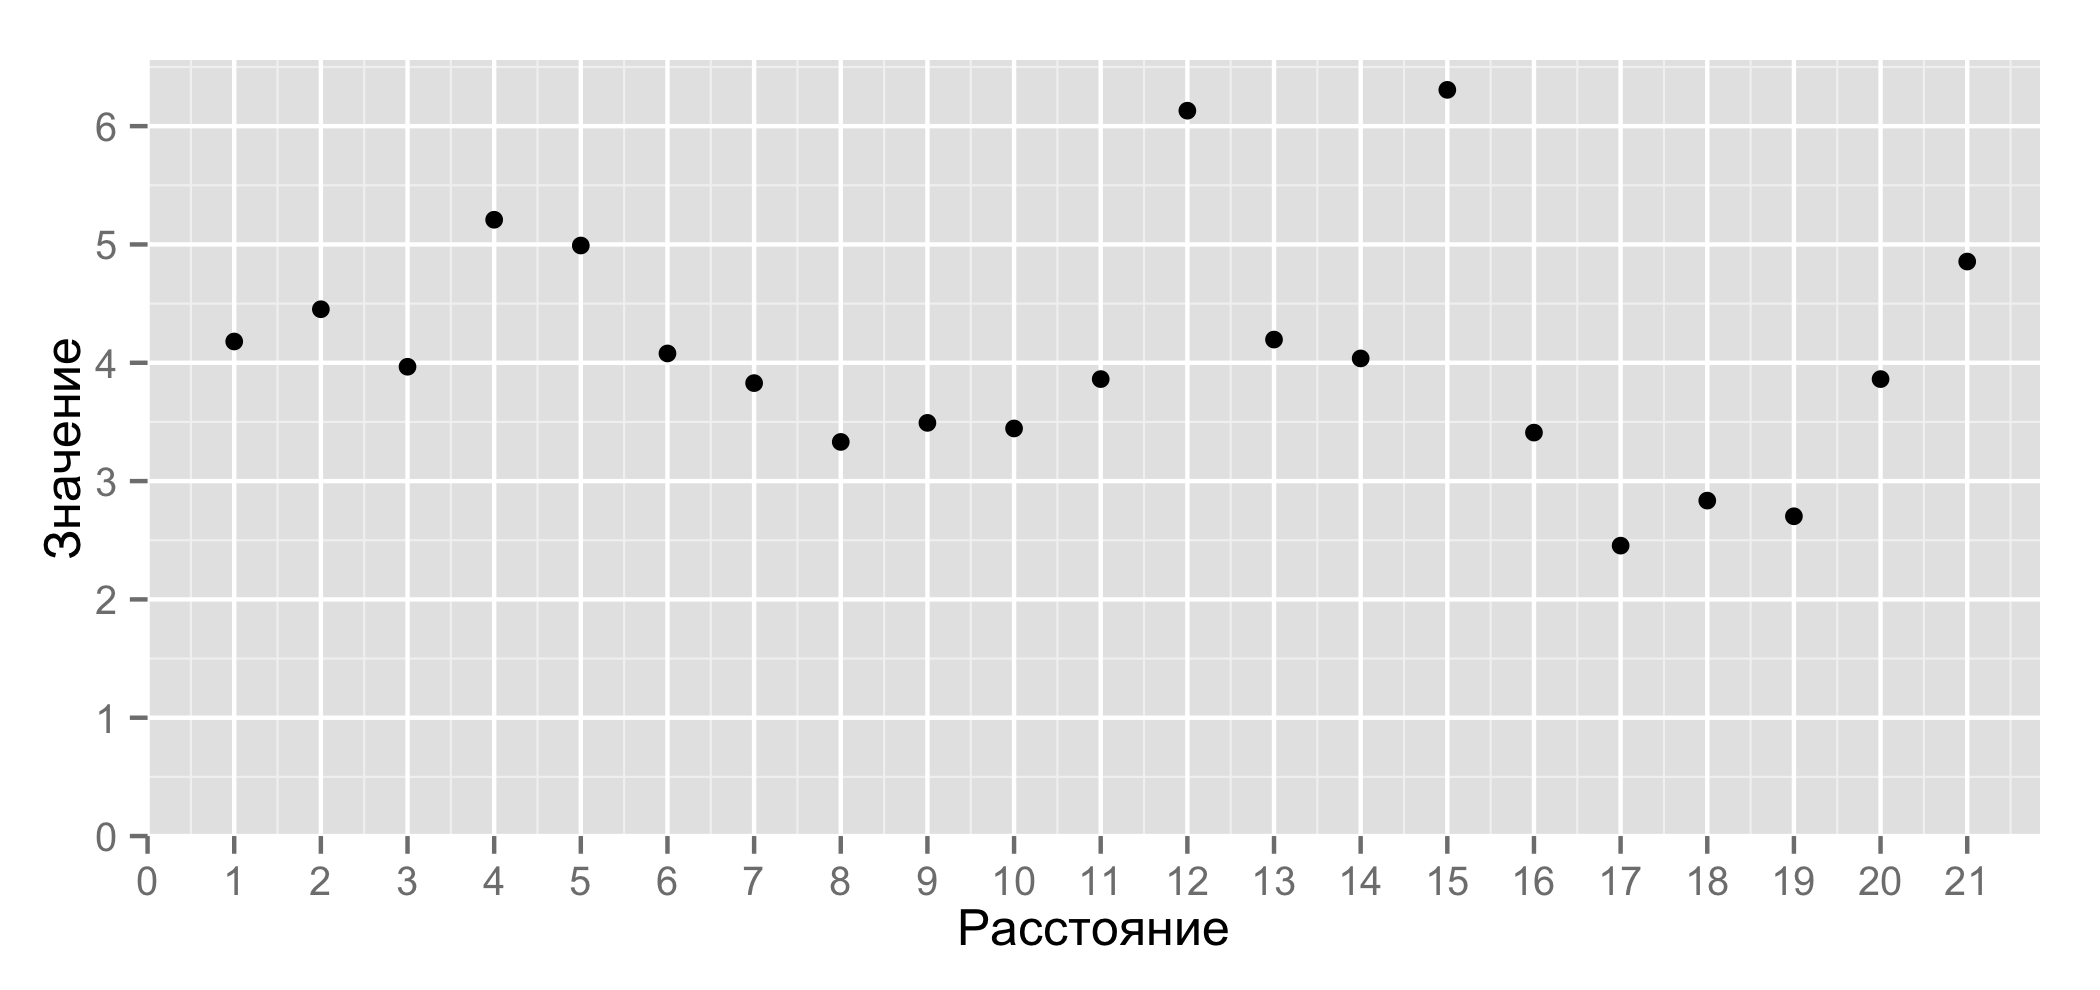
\includegraphics[width=1\linewidth]{../figures/variogram/lin-variogram.png}}
\caption{Оценка семивариограммы Матерона}
\label{img:variogram}
\end{figure}

На практике построение модели семивариограммы представляет собой итеративный процесс, на каждом шаге которого следует наилучшим образом подобрать параметры очередного модельного приближения. При этом существует два пути подбора моделей семивариограммы: подбор силами исследователя, т.е. визуально с ручным выбором параметров, и автоматическим подбором параметров с помощью специальных методов и алгоритмов. В различных источниках рекомендуется строить модели вручную, так как исследователь лучше знает специфику данных и может учесть это при подборе параметров \cite{geostat2010}. Исследуем оба подхода: визуальный и автоматический подбор параметров.

Следует также отметить, что в некоторых источниках советуют при построении модели семивариограммы учитывать параметр максимального расстояния, до которого вычисляются значения семивариограммы, а также приводят рекомендацию по его подбору. В связи с этим, первоначальным параметром было выбрано значение, рассчитанное по рекомендации \cite{cressie2011statistics}:
\begin{equation}
\label{eq:cutoff}
	h_{\text{max}} = 2n / 3 = 20
\end{equation}
При таком значении можно наблюдать все особенности семивариограммы и не рассматривать отдаленные значения.

Вследствие выводов по диаграмме взаимного разброса, начнём подбор модели семивариограммы с линейной модели \eqref{eq:lin}. Подбор начальных параметров осуществим визуально. Из уравнения \eqref{eq:lin} видно, что параметр $ b $ отвечает за угол наклона прямой, поэтому примем начальное значение $ b = 4 $, приблизительно равное дисперсии. Построенная модель, вида
\begin{equation*}
	\widehat{\gamma}_1(h) = Lin(h), \quad b = 4,
\end{equation*}
отображена на графике \ref{img:lin-modeled}. Следует отметить, что данная модель после применения кригинга позволила получить значения очень близкие к нулю, что не изменило прогноза, построенного по модели тренда (таблица \ref{table:prediction_trend}).

Далее подберём модель семивариограммы с помощью возможностей пакета \textit{gstat}. В результате его использования получаем модель $ \widehat{\gamma}_2(h) $ с чистым эффектом самородков
\begin{equation}
\label{eq:nug}
	\gamma(h) = c \cdot Nug(h) = \left\{
 \begin{array}{l l}
   0, & h = 0, \\
   c, & h \neq 0,
 \end{array} \right.
\end{equation}
с параметром $ c = \characteristic{variogram}{lin-fit-nug} $. Объяснить такой результат можно тем, что автоматический подбор параметров из пакета \textit{gstat} основан на методе наименьших квадратов. А поскольку значения семивариограммы сразу достигают порогового значения, приблизительно равному дисперсии, то эффект самородков $ \widehat{\gamma}_2(h) $, изображённый на рисунке \ref{img:lin-fit}, оказывается наилучшей моделью. Но при этом данная модель не учитывает особенностей исследуемых данных, поэтому результатов прогнозирования она не улучшила (таблица \ref{table:lin-fit-prediction}, приложение \ref{c:app_results}). Другими словам, данный подход не учитывает поведение оценки семивариограммы около нуля, поскольку в исходных данных нет информации о ближайших к исследуемому месяцах.

Наличие порога объяснимо видом оценки семивариограммы: на рисунке \ref{img:variogram}, как уже было замечено, уже первые значения достигают уровня дисперсии. И отклонение от этого значения не велико. Это согласуется с результатами, полученными при анализе остатков. Из этого следует, что использование только беспороговых моделей не обосновано. При этом следует учесть то, что не учёл автоматический подбор параметров: поведение $ \tilde{\gamma}(h) $ около нуля. Поэтому воспользуемся линейной моделью с порогом \eqref{eq:linsill}, которая является комбинацией моделей \eqref{eq:lin} и \eqref{eq:nug} \cite{pebesma2001gstat}.
\begin{equation}
\label{eq:linsill}
	\widehat{\gamma}(h) = c_0 + c \cdot Lin(h, a) = \left\{
 \begin{array}{l l}
   c_0 + c \cdot \frac{h}{a}, & 0 \leq h \leq a, \\
   c_0 + c, & h > a,
 \end{array} \right.
\end{equation}
где $ c_0 $ -- эффект самородков, $ c $ -- порог, $ a $ -- ранг.

Для подбора оптимальных параметров модели семивариограммы \eqref{eq:linsill} воспользуемся инструментами реализованной программы, рассмотренной в главе 3. Воспользуемся первым из описанных подходом --- перекрёстным. В качестве статистики, для оценки качества модели, будем использовать коэффициент корреляции между $ \varepsilon(t) $ и $ \varepsilon^{*}(t)$ . График зависимости значения ранга на качество модели отображён на рисунке \ref{img:lin-range-cv}.
\begin{figure}[ht]
	\center{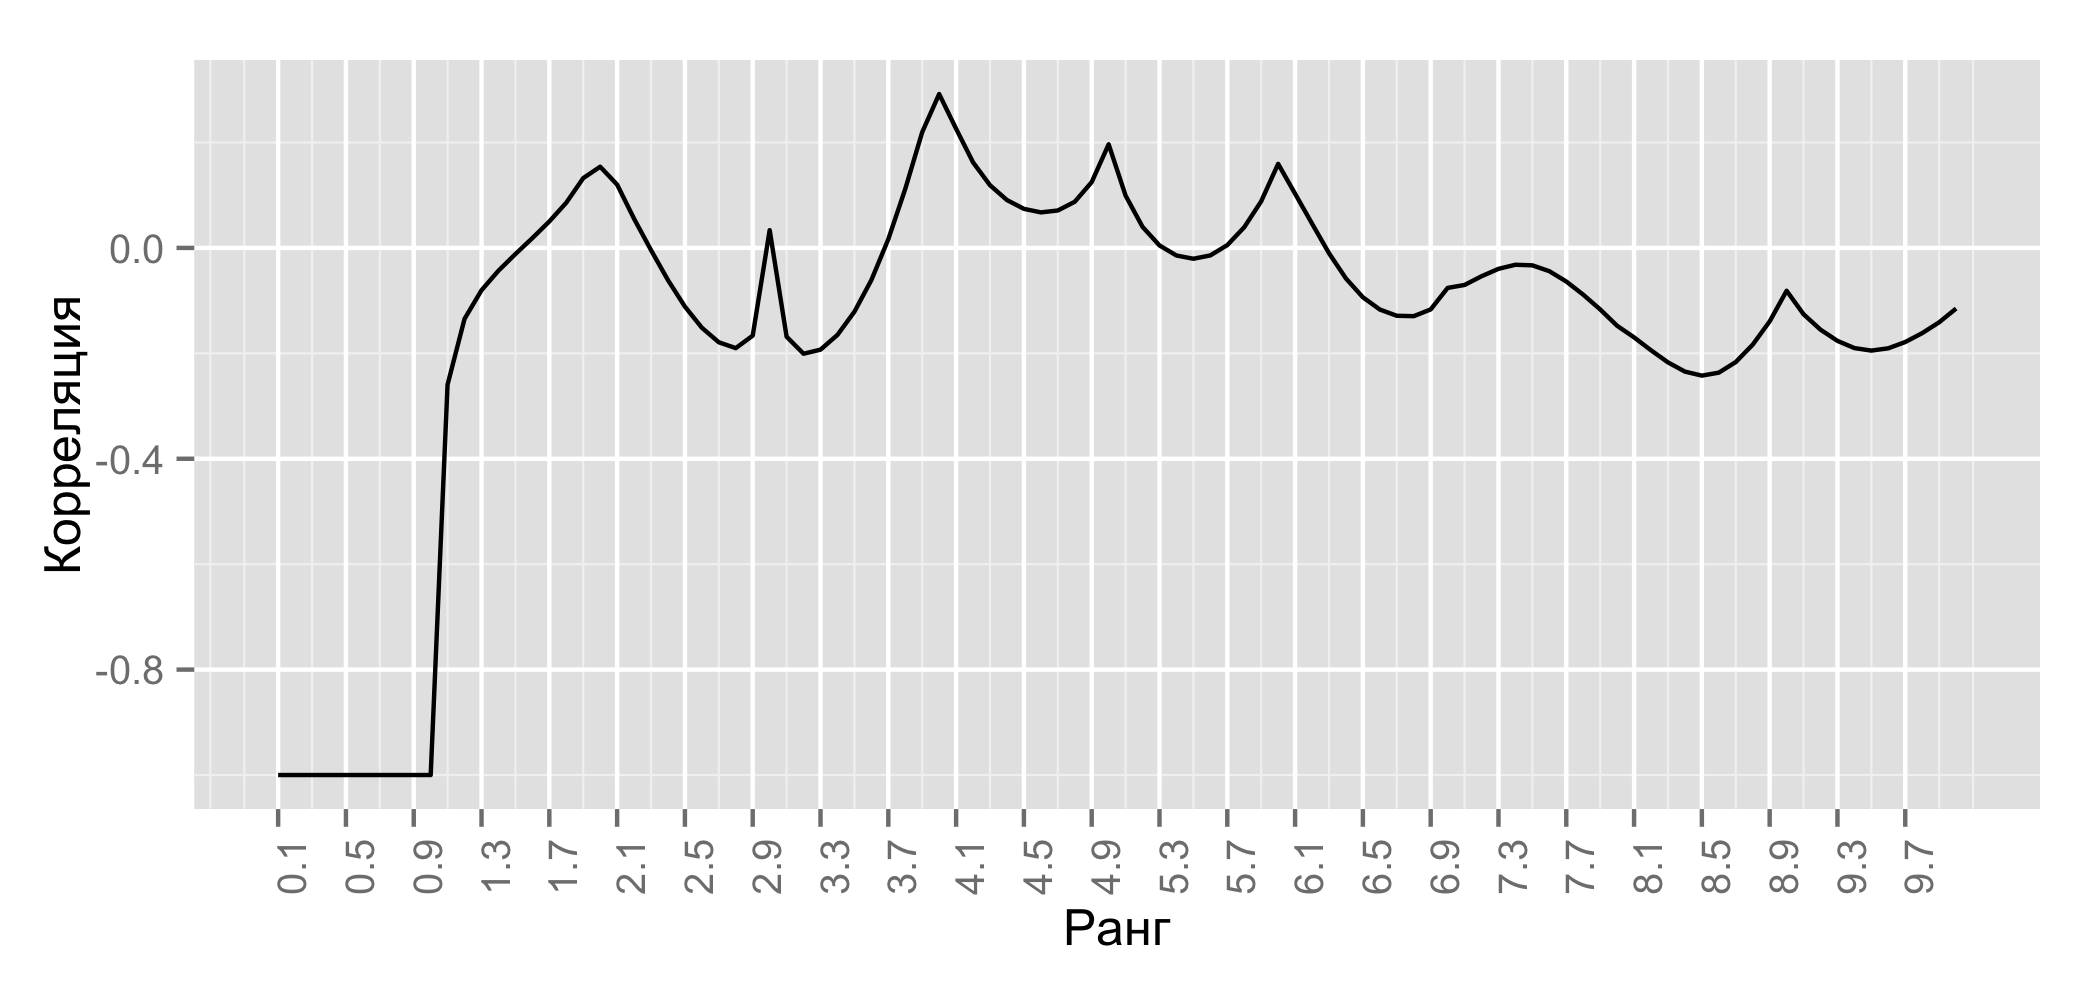
\includegraphics[width=1\linewidth]{../figures/variogram/lin-range-corr.png}}
\caption{Зависимость качества линейной модели от значения ранга}
\label{img:lin-range-cv}
\end{figure}
По рисунку видно, что максимальное значение коэффициента корреляции $ r_{\varepsilon\varepsilon^{*}} = 0.292 $ достигается при значении ранга $ a = 4 $. Таким образом получена модель
\begin{equation}
\label{eq:gamma3}
 	\widehat{\gamma}_3(h) = 4 \cdot Lin(h, 4),
\end{equation}
её график отображен на рисунке \ref{img:lin-fit-cv}. Вычисленные по данной модели прогнозные значения можно проследить по таблице \ref{table:lin-fit-cv-prediction} и по графику \ref{img:lin-fit-cv-pred} в приложении \ref{c:graphs}. Прогнозные значения оказались не очень точными, что объясняется высоким значением среднеквадратической ошибки \eqref{eq:mse} ($ MSE = 7.931 $). При этом, коэффициент корреляции $ r_{\varepsilon\varepsilon^{*}} = 0.292 $ выше, чем аналогичные коэффициенты корреляции уже построенных моделей. Поэтому можно сделать вывод о том, что данная модель может использоваться для описания исходных данных, в частности, для вычислений пропущенных наблюдений.

% latex table generated in R 3.1.3 by xtable 1.7-4 package
% Sat May 30 20:32:50 2015
\begin{table}[H]
\centering
\begin{tabular}{r|cccc}
  \hline
 & $X(t)$ & $X^{*}(t)$ & $y(t)$ & $ X(t) - X^{*}(t) $ \\ 
  \hline
2007 & 19.400 & 20.824 & 21.578 & -1.424 \\ 
  2008 & 21.800 & 21.133 & 21.687 & 0.667 \\ 
  2009 & 21.900 & 19.831 & 21.797 & 2.069 \\ 
  2010 & 24.300 & 22.129 & 21.906 & 2.171 \\ 
  2011 & 22.800 & 22.239 & 22.016 & 0.561 \\ 
  2012 & 20.200 & 22.348 & 22.126 & -2.148 \\ 
   \hline
\end{tabular}
\caption{Прогнозные значения (модель $ \widehat{\gamma}_3(h) $)} 
\label{table:lin-fit-cv-prediction}
\end{table}


Для построения более точного прогноза воспользуемся адаптивным подходом по подбору параметров, который введён в главе 3. График зависимости среднеквадратической ошибки от ранга при таком подходе отображен на рисунке \ref{img:lin-range-adapt}. Оптимальным параметром для ранга, из этого графика, является значение $ a = 2 $, с минимальной среднеквадратической ошибкой $ MSE = 1.62 $.
\begin{equation}
\label{eq:gamma4}
 	\widehat{\gamma}_4(h) = 4 \cdot Lin(h, 2).
\end{equation}

Построенная модель семивариограммы \eqref{eq:gamma4} изображена на рисунке \ref{img:lin-adapt-modeled}. График \ref{img:lin-adapt-pred}
\begin{figure}[ht]
	\center{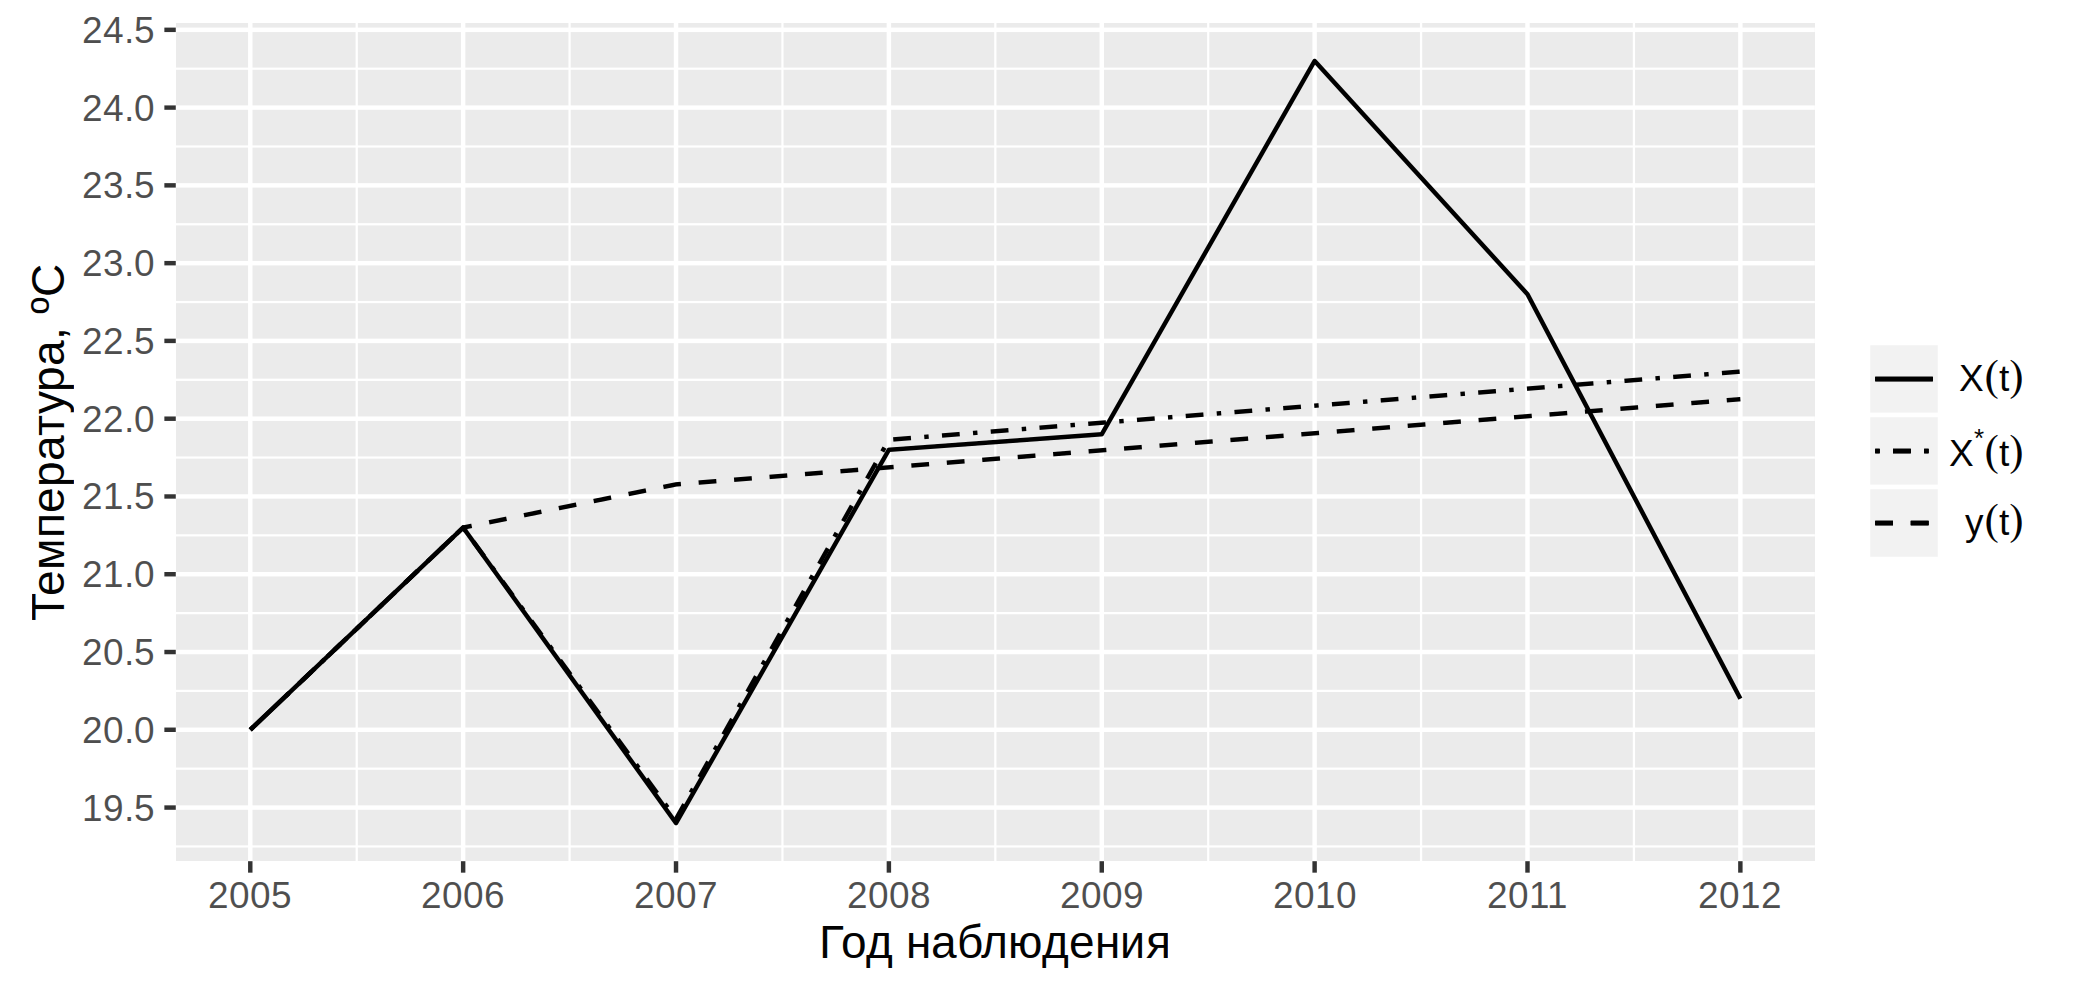
\includegraphics[width=1\linewidth]{../figures/variogram/lin-fit-adapt-cross-prediction.png}}
\caption{Прогноз по модели $ \widehat{\gamma}_4(h) $}
\label{img:lin-adapt-pred}
\end{figure}
и таблица \ref{table:lin-fit-adapt-prediction} прогнозных значений показывают, что данный подход позволил получить значения за $ 2007 $--$ 2009 $ годы очень близкие к исходным. Что является хорошим результатом. При этом статистики по данной модели после проведения кросс-валидации оказались равными: коэффициент корреляции $ r_{\varepsilon\varepsilon^{*}} = 0.152 $, среднеквадратическая ошибка $ MSE = 18.69 $. Что говорит о том, что данная модель описывает всю выборку хуже чем предыдущая. Таким образом модель, полученная адаптивным подбором параметров хорошо себя показывает для вычисления краткосрочных значений, в свою очередь перекрёстный метод может применяться для нахождения модели, описывающей наилучшим образом исходные данные.

%TODO Таким образом можно сделать выводы о преимуществах продемонстрированных подходов. Недостаток первого подхода заключается в том, что модель, описывающая поведение исследуемых данных сглаживает локальное поведение, вследствие чего прогнозные значения могут получиться не всегда точными. В рамках рассматриваемой задачи, когда данные имеют сложную структуру, потеря информации о локальных изменениях в значениях, влечёт ухудшение прогноза. Во втором же случае, в отличие от первого, описывается поведение не всей выборки, а только те, которые интересны больше всего --- последние наблюдения, так как они в большей мере влияют на будущие значения. Но в этом случае учитывается в меньшей степени поведение данных в целом.

Модель $ \widehat{\gamma}_4(h) $, полученная адаптивным подходом, как было упомянуто ранее, описывает исходные данные не очень точно. Поэтому есть необходимость в поиске моделей, дающих лучшие результаты. Одной из самых распространённых и часто используемой пороговой моделью является сферическая \cite{geostat2010}:
\begin{equation*}
	\widehat{\gamma}(h) = c_0 + c \cdot Sph(h, a) = \left\{
		\begin{array}{l l}
			c_0 + c \cdot (\frac{3}{2} \frac{h}{a} - \frac{1}{2}(\frac{h}{a})^3), & h \le a, \\
			c_0 + c, & h \geq a.
		\end{array} \right.
\end{equation*}
Однако после подбора оптимальных параметров оказалось, что данная модель вписывается в исследуемые данные хуже, чем найденные ранее. При перекрёстном подборе параметров наилучшей получилась модель
\begin{equation}
\label{eq:gamma5}
	\widehat{\gamma}_5(h) = 4 Sph(h, 2.3),
\end{equation}
с показателями качества: коэффициент корреляции $ r_{\varepsilon\varepsilon^{*}} = -0.002$ и среднеквадратической ошибкой $ MSE = 5.407$. В случае адаптивного подхода, оптимальными оказались параметры $ c = 4, a = 6.9 $ c эффектом самородков равным $ 0.9 $, со среднеквадратической ошибкой прогнозных и истинных значений $ MSE = 2.01 $. Применив кросс-валидацию к этой модели, получаем следующие показатели качества: коэффициент корреляции $ r_{\varepsilon\varepsilon^{*}} = -0.009 $ и среднеквадратической ошибкой $ MSE = 5.396 $. Графики семивариограммы и прогнозных значений последней модели отображены на рисунках \ref{img:sph-adapt-modeled} и \ref{img:sph-adapt-pred} в приложении \ref{c:graphs} соответственно. Можно сделать вывод, что как и модель $ \widehat{\gamma}_4(h) $ \eqref{eq:gamma4}, сферическая модель $ \widehat{\gamma}_5(h) $ не позволила описать поведение исследуемой выборки. Только в случае краткосрочного прогноза она проявила себя, предсказав характерное поведение исключённых значений, хоть и хуже модели $ \widehat{\gamma}_4(h) $. Полученный результат является следствием вида их моделей семивариограммы. На их графиках \ref{img:lin-adapt-modeled} и \ref{img:sph-adapt-modeled} в приложении \ref{c:graphs} можно видеть, что они похожи: линейное поведение до значения порога, и прямая линия, отвечающая за некоррелированные значения, на его уровне. Как следствие, похожие результаты.

Если обратить внимание на график экспериментальной семивариограммы \ref{img:variogram}, то можно заметить некоторый периодический эффект в виде волны. Поэтому дальнейшей подбираемой моделью возьмем периодическую \cite{pebesma2001gstat}:
\begin{equation}
\label{eq:per}
	\widehat{\gamma}(h) = c_0 + c \cdot Per(h, a) = 1 - cos(\frac{2 \pi h}{a}),
\end{equation}
где $ c_0 $ -- эффект самородков, $ c $ -- порог, $ a $ -- ранг.

С помощью перекрёстного метода в написанной программе подобрана модель
\begin{equation}
\label{eq:gamma6}
	\widehat{\gamma}_6(h) = 4 \cdot Per(h, 0.898),
\end{equation}
график семивариограммы которой изображен на рисунке \ref{img:per-cv-modeled} в приложении \ref{c:graphs}. Показатели качества подобранной модели: коэффициент корреляции $ r_{\varepsilon\varepsilon^{*}} = 0.404 $, среднеквадратическая ошибка $ MSE = 4.369 $. Следует отметить, что из всех подбираемых моделей, представленное значение коэффициента корреляции оказалось самым большим. Что говорит о том, что данная модель наилучшим образом описывает исследуемые данные. Таблица \ref{table:per-fit-cv-prediction} в приложении \ref{c:app_results} и график прогнозных значений \ref{img:per-cv-pred}
\begin{figure}[ht]
	\center{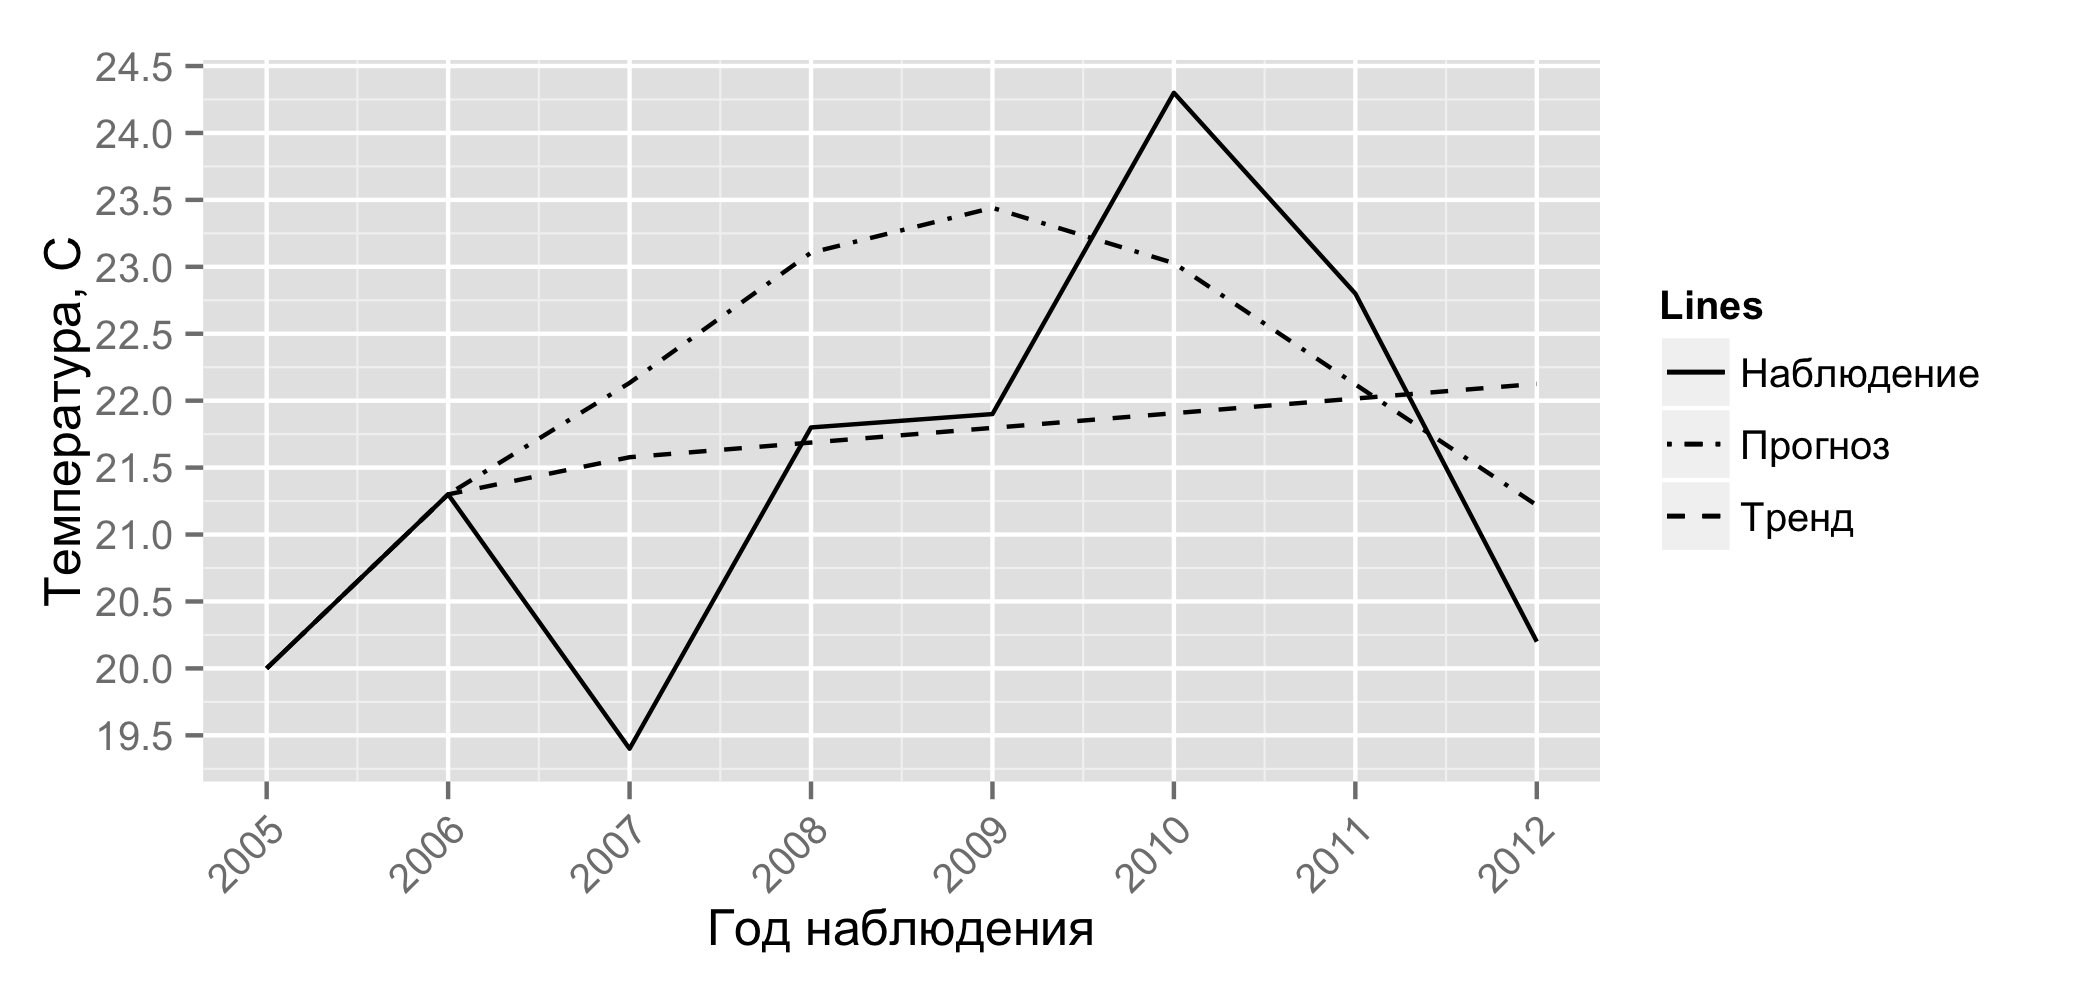
\includegraphics[width=1\linewidth]{../figures/variogram/per-fit-cv-cross-prediction.png}}
\caption{Прогноз по модели $ \widehat{\gamma}_6(h) $}
\label{img:per-cv-pred}
\end{figure}
по подобранной модели \eqref{eq:gamma6} показывают, что прогноз получился не очень точный, но при этом следует принять во внимание, что данная модель подбиралась для описания всей выборки, не учитывая локальное поведение в последних наблюдениях. Модель $ \widehat{\gamma}_6(h) $ оказалась наилучшей для описания всей выборки из всех проверенных.

%TODO: Следует отметить, что инструменты используемой программы позволяют относительно быстро проверить различные модели на практике.

Следует также упомянуть использовавшуюся оценку семивариограммы Кресси-Хокинса \eqref{eq:cressie}. Она изображена на рисунке \ref{img:robust-variogram} в приложении \ref{c:graphs}. По характерным особенностям данная модель не сильно отличается от оценки Матерона \eqref{eq:var_estimation}, поэтому на результаты подбора моделей визуальным подходом она не повлияла.

Таким образом, с помощью инструментов реализованной программы проанализированы различные модели семивариограмм и влияние их параметров на результаты прогноза. Подбор осуществлён двумя методами: перекрёстным и адаптивным. С их помощью найдены наилучшие модели: перекрёстным методом подбора найдена периодическая модель $ \widehat{\gamma}_6(h) $, адаптивным --- линейная с порогом $ \widehat{\gamma}_4(h) $. Как следствие, метод перекрёстный метод подбора параметров следует использовать для решения задач описания исследуемых данных, адаптивный --- для решения задач по построению точных краткосрочных прогнозов.

% subsection _variogram (end)

\subsection{Автоматический подход} % (fold)
\label{sec:autovar}

%TODO: так как визуальный подход, как было показано ранее, требует определённых знаний и усилий, появляется 

Как было отмечено, существуют также автоматические методы подбора моделей и параметров специальными метода и алгоритмами. В рамках данной работы был реализован алгоритм, основанный на возможностях пакета \textit{gstat}, позволяющий автоматически выбирать наилучшую. Подбор параметров определённой модели семивариограммы осуществляется методом наименьших квадратов, пример использования которого показан ранее (для модели $ \gamma_2(h) $). Подбор параметров сопровождается невязкой модели и значений семивариограммы. Это позволяет, основываясь на данном показателе, выбирать наилучшим образом подходящей модели --- по минимальному значению невязки. Следует отметить, что в данном случае параметр максимального расстояния $ h_{\text{max}} $, для которого вычисляется семивариограмма, будет проявлять себя при выборе модели, поскольку количество точек, по которым подбирается модель, будет влиять на метод наименьших квадратов. Исходный код функции, реализующей автоматический подбор моделей, представлен в листинге \ref{lst:afv}.

Воспользуемся автоматическим методом подбора модели для оценки Матерона. Данная процедура, при принятом ранее максимальном значении лага \eqref{eq:cutoff}, выбрала волновую модель \eqref{eq:wave} семивариограммы с эффектом самородков:
\begin{equation}
\label{eq:wave}
	\widehat{\gamma}(h) = c_0 + c \cdot Wav(h, a) = 1 - \frac{a}{h} \cdot sin(\frac{h}{a}),
\end{equation}
где $ c_0 $ -- эффект самородков, $ c $ -- порог, $ a $ -- ранг.

Обозначим полученную модель
\begin{equation}
\label{eq:gamma7}
	\widehat{\gamma}_7(h) = 3.03 + 1.011 \cdot Wav(h, 1.14),
\end{equation}
графически подобранная модель и прогноз, построенный на её основе с применением кригинга, отображены на рисунках \ref{img:auto-class-modeled} и \ref{img:auto-class-20-pred} соответственно. По которым видно, что результат получился значительно хуже результатов по моделям, найденных ранее. При этом показатели качества оказались равными: коэффициент корреляции $ r_{\varepsilon\varepsilon^{*}} = -0.2 $ и среднеквадратическая ошибка $ MSE = 4.155 $. Что подтверждает выводы по графикам.

Так как параметр $ h_{\text{max}} $ влияет на подбор моделей семивариограммы, оценим качество моделей, подобранных автоматически, в зависимости от него. Как и ранее, качество модели будем оценивать двумя подходами: перекрёстным и адаптивным. Первый случай отображен на рисунке \ref{img:auto-corr-cutoff}. Как видно из него, наибольший коэффициент корреляции соответствует оценке Матерона и максимальному расстоянию $ h_{\text{max}} = 26 $.
\begin{figure}[ht]
	\center{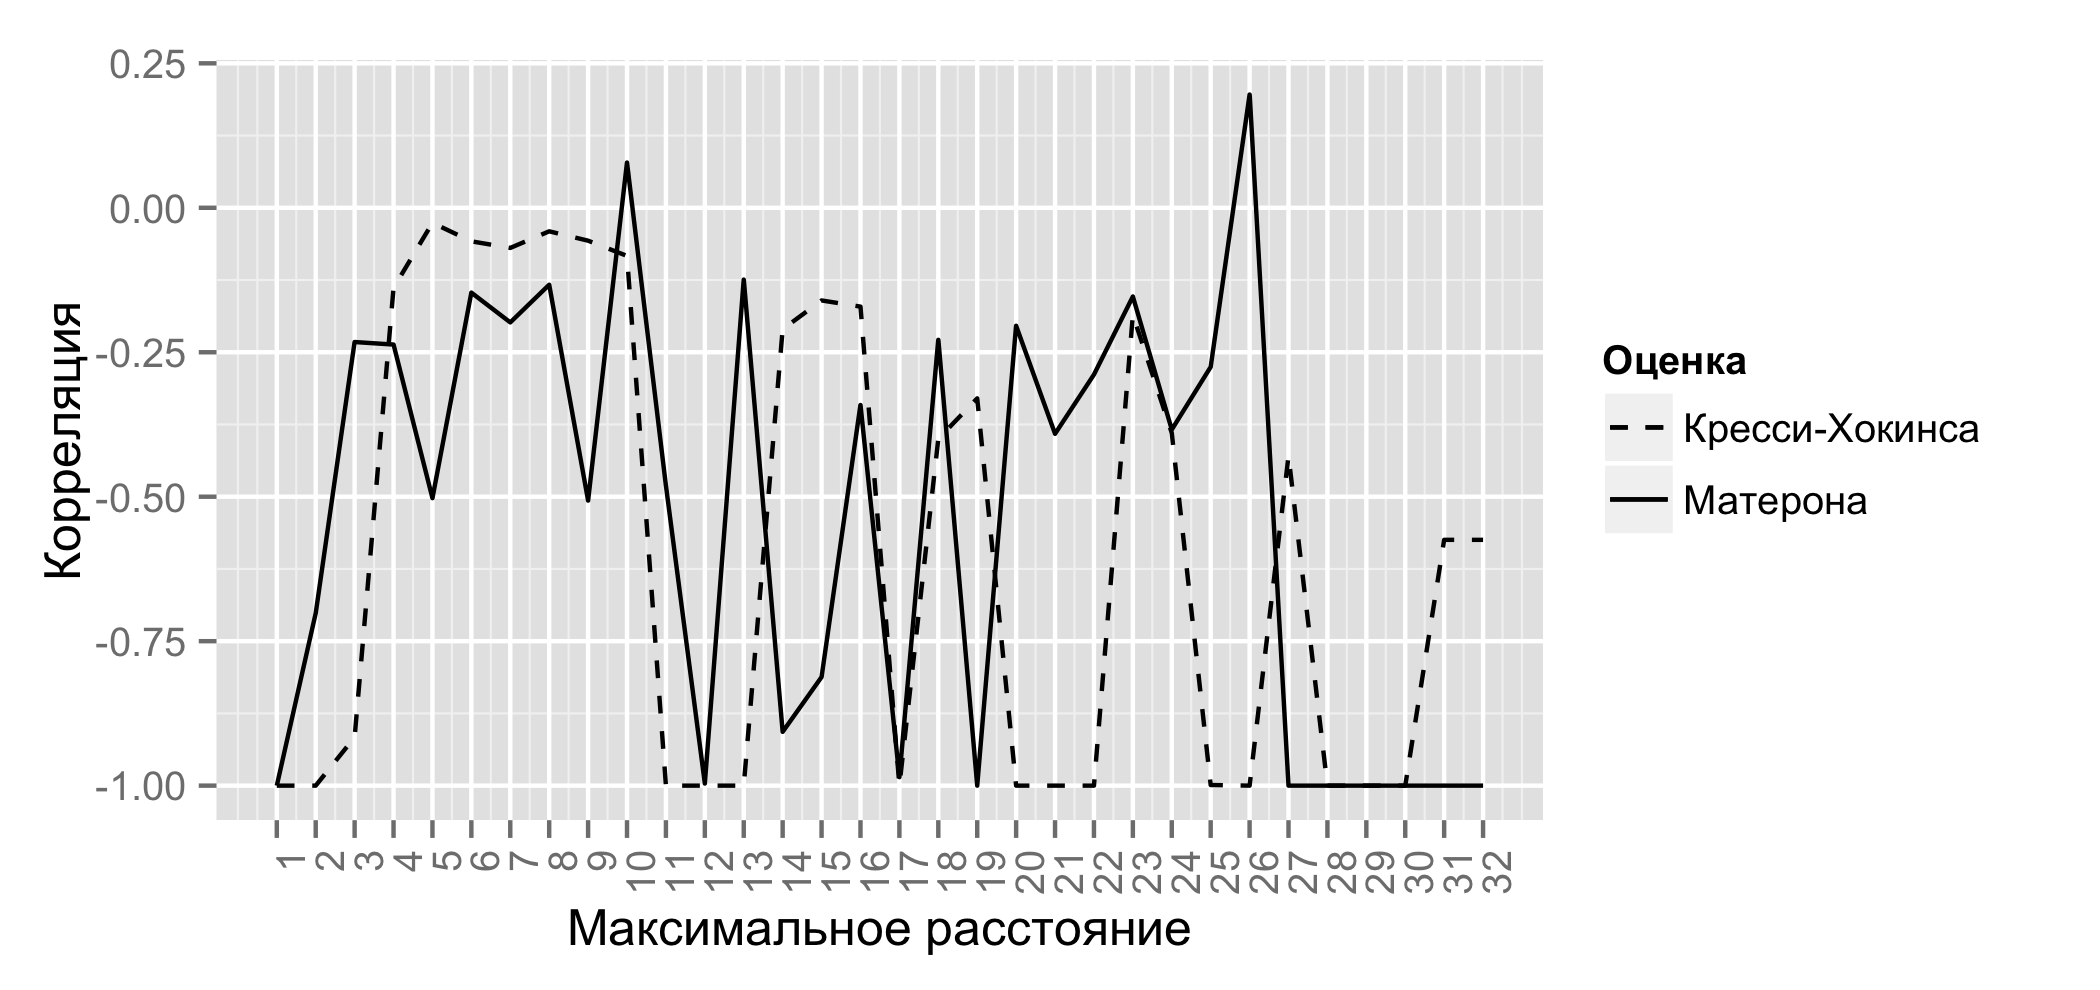
\includegraphics[width=1\linewidth]{../figures/variogram/auto-corr-cutoff.png}}
\caption{Зависимость качества модели от максимального расстояния}
\label{img:auto-corr-cutoff}
\end{figure}
Для найденного значения $ h_{\text{max}} $, наилучшей моделью является периодическая \eqref{eq:per}:
\begin{equation*}
 	\widehat{\gamma}_8(h) = 3.46 + 0.5 \cdot Per(h, 2.67),
\end{equation*}
с показателями качества: коэффициент корреляции $ r_{\varepsilon\varepsilon^{*}} = 0.196 $, среднеквадратической ошибкой $ MSE = 3.835 $. График прогнозных значений отображён на рисунке \ref{img:auto-class-26-pred}. Таким образом, автоматическим способом найдена модель, которая была получена ранее вручную. Отличие заключается только в значениях параметров. В случае автоматического подбора, модель хуже описывает поведение исходных данных. Но при этом следует учитывать затраты на поиск той или иной модели в обоих случаях.

Также проследим зависимость значения максимального расстояния при адаптивном подходе. График такой зависимости изображен на рисунке \ref{img:auto-mse-cutoff}.
\begin{figure}[ht]
	\center{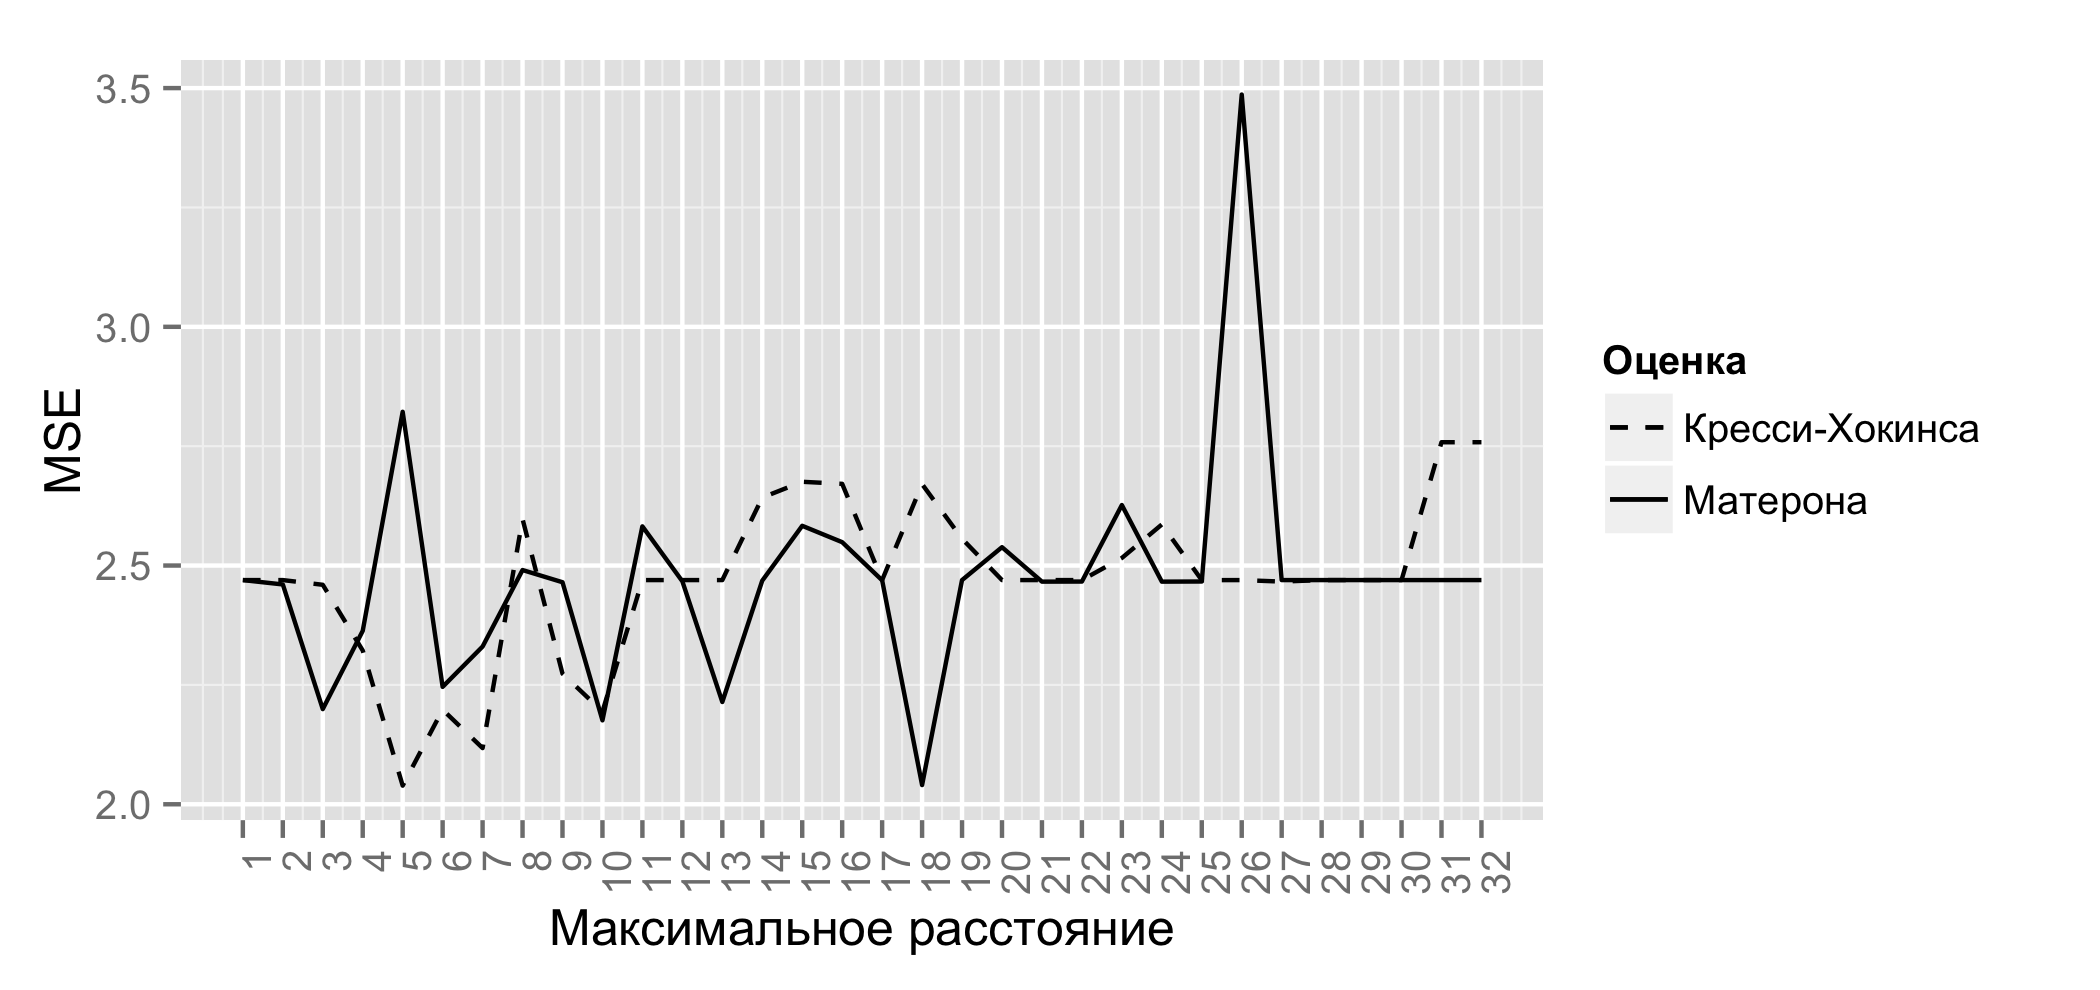
\includegraphics[width=1\linewidth]{../figures/variogram/auto-mse-cutoff.png}}
\caption{Зависимость качества модели от максимального расстояния}
\label{img:auto-mse-cutoff}
\end{figure}
В данном случае, оптимальной моделью оказалась волновая модель с эффектом самородков
\begin{equation*}
 	\widehat{\gamma}_9(h) = 4.11 + 1.65 \cdot Wav(h, 3.59),
\end{equation*}
полученная по оценке Кресси-Хокинса при значении максимального расстояния $ h_{\text{max}} = 5 $. И при почти равном значении среднеквадратической ошибки, периодическая модель с эффектом самородков
\begin{equation*}
 	\widehat{\gamma}_{10}(h) = 3.8 + 0.32 \cdot Per(h, 1.3)
\end{equation*}
по оценке Матерона при значении максимально расстояния $ h_{\text{max}} = 18 $. Прогнозные значения первой и последней можно проследить по таблице \ref{table:auto-rob-5-prediction} в приложении \ref{c:app_results} и таблице \ref{table:auto-class-18-prediction} соответственно. А также графически на рисунках \ref{img:auto-rob-5-pred} и \ref{img:auto-class-18-pred}.

% latex table generated in R 3.1.3 by xtable 1.7-4 package
% Sat May 30 20:33:23 2015
\begin{table}[ht]
\centering
\begin{tabular}{r|cccc}
  \hline
 & $X(t)$ & $X^{*}(t)$ & $y(t)$ & $ X(t) - X^{*}(t) $ \\ 
  \hline
2007 & 19.400 & 21.170 & 21.578 & -1.770 \\ 
  2008 & 21.800 & 21.553 & 21.687 & 0.247 \\ 
  2009 & 21.900 & 22.151 & 21.797 & -0.251 \\ 
  2010 & 24.300 & 22.078 & 21.906 & 2.222 \\ 
  2011 & 22.800 & 21.665 & 22.016 & 1.135 \\ 
  2012 & 20.200 & 21.860 & 22.126 & -1.660 \\ 
   \hline
\end{tabular}
\caption{Прогнозные значения (модель $ \widehat{\gamma}_{10}(h) $)} 
\label{table:auto-class-18-prediction}
\end{table}

Как можно видеть, представленные прогнозные значения далеки от истины. Но при этом поведение исходных данных найденные модели уловили. Что является хорошим результатом, если учитывать специфичность рассматриваемой задачи. Было показано, что метод наименьших квадратов не учитывает особенностей, которые может учесть исследовать. А так как в данной задаче может присутствовать множество неучтённых факторов, то применение автоматического подбора моделей предсказуемо показывает результаты хуже. Данный метод подбора моделей может быть обоснованно использован в случае данных, изменение которых носят плавный характер. К примеру, уровень воды некоторого озера. Или, использовать для анализа данные, наблюдения в которых будут располагаться ближе, чем годовой промежуток. Так как температура воды в конкретном месяце скорее будет зависеть от температуры воды предыдущего месяца, чем от температуры воды в рассматриваемый месяц год назад.

Для сравнения всех построенных моделей по показателям качества, использовался сводная таблица \ref{table:summary-cv}.
% latex table generated in R 3.1.3 by xtable 1.7-4 package
% Tue Jun  2 18:00:13 2015
\begin{table}[ht]
\centering
\caption{Сводная таблица показателей качества моделей семивариограмм}
\label{table:summary-cv}
{\footnotesize
\begin{tabular}{r|cccccccccc}
  \hline
 & $ \widehat{\gamma}_1(h) $ & $ \widehat{\gamma}_2(h) $ & \boldmath$ \widehat{\gamma}_3(h) $ & $ \widehat{\gamma}_4(h) $ & $ \widehat{\gamma}_5(h) $ & \boldmath$ \widehat{\gamma}_6(h) $ & $ \widehat{\gamma}_7(h) $ & $ \widehat{\gamma}_8(h) $ & $ \widehat{\gamma}_9(h) $ & $ \widehat{\gamma}_{10}(h) $ \\ 
  \hline
$ S $ & 202.36 & 134.38 & \textbf{253.80} & 598.03 & 172.66 & \textbf{108.19} & 132.97 & 122.72 & 141.62 & 167.00 \\ 
  $ E $ & 1.60 & 1.07 & \textbf{2.01} & 4.74 & 1.37 & \textbf{0.86} & 1.05 & 0.97 & 1.12 & 1.32 \\ 
  $ MAE $ & 2.22 & 1.76 & \textbf{2.42} & 4.00 & 2.01 & \textbf{1.42} & 1.72 & 1.67 & 1.74 & 1.98 \\ 
  $ MSE $ & 6.32 & 4.20 & \textbf{7.93} & 18.69 & 5.40 & \textbf{3.38} & 4.16 & 3.84 & 4.43 & 5.22 \\ 
  $ r_{\varepsilon\varepsilon^{*}} $ & -0.09 & -0.04 & \textbf{0.29} & 0.15 & -0.09 & \textbf{0.40} & -0.20 & 0.20 & -0.03 & -0.15 \\ 
   \hline
\end{tabular}
}
\end{table}


В свою очередь, в таблице \ref{table:summary-prediction} наглядно представлены полученные с помощью каждой из моделей прогнозные значения.
% latex table generated in R 3.1.3 by xtable 1.7-4 package
% Tue Jun  2 14:46:09 2015
\begin{table}[ht]
\centering
\caption{Сводная таблица реальных $ X(t)$ и прогнозных $ X_i^{*}(t), i=~\overline{1,10} $ значений} 
\label{table:summary-prediction}
{\footnotesize
\begin{tabular}{r|rcccccccccc}
  \hline
Год & X(t) & $ X^{*}_1(t) $ & $ X^{*}_2(t) $ & $ X^{*}_3(t) $ & \boldmath$ X^{*}_4(t) $ & $ X^{*}_5(t) $ & $ X^{*}_6(t) $ & $ X^{*}_7(t) $ & $ X^{*}_8(t) $ & $ X^{*}_9(t) $ & $ X^{*}_{10}(t) $ \\ 
  \hline
  2007 & 19.40 & 21.41 & 21.58 & 20.82 & \textbf{19.43} & 21.29 & 22.13 & 21.64 & 22.42 & 21.38 & 21.17 \\ 
  2008 & 21.80 & 21.52 & 21.69 & 21.13 & \textbf{21.86} & 21.71 & 23.11 & 21.61 & 21.18 & 21.88 & 21.55 \\ 
  2009 & 21.90 & 21.63 & 21.80 & 19.83 & \textbf{21.97} & 22.15 & 23.44 & 21.89 & 21.66 & 22.16 & 22.15 \\ 
  2010 & 24.30 & 21.74 & 21.91 & 22.13 & \textbf{22.08} & 22.32 & 23.03 & 21.82 & 22.60 & 22.22 & 22.08 \\ 
  2011 & 22.80 & 21.85 & 22.02 & 22.24 & \textbf{22.19} & 22.29 & 22.12 & 22.09 & 21.18 & 22.13 & 21.66 \\ 
  2012 & 20.20 & 21.96 & 22.13 & 22.35 & \textbf{22.30} & 22.29 & 21.22 & 22.08 & 22.62 & 22.05 & 21.86 \\ 
   \hline
\end{tabular}
}
\end{table}


Следует также отметить, что применение оценки Кресси-Хокинса дало результат лишь в случае автоматического подбора параметров. На визуальный подбор модели она никак не повлияла. Что обосновано ее назначением и показанным отсутствием выбросов в исследуемых данных.

Таким образом в результате вариограммного анализа были исследованы различные модели семивариограмм, проанализированы оценки Матерона и Кресси-Хокинса, исследованы два подхода по оценке качества модели и подбору моделей и параметров. Как следствие, в рамках рассматриваемой задачи, можно рекомендовать использование перекрёстный метод подбора параметров  для вычисления прогнозных значений и адаптивный метод для описания исследуемых данных. И соответствующие модели, найденные этими методами: линейной модели с порогом вида \eqref{eq:linsill} и периодической модели вида \eqref{eq:per}. Следует также отметить, что автоматический метод подбора моделей в рассматриваемых условиях показал результаты хуже, чем визуальный подбор. Но в условиях, когда нужно быстро оценить какие-либо данные, данный метод может оказаться очень полезным. Также, автоматический метод может использоваться для данных, изменение которых имеет более плавный характер. В других случаях, следуют применять визуальных подход по выбору моделей и параметров, поскольку он позволяет наиболее точно учесть все факторы и, как следствие, получить наилучший результат.

% subsection autovar (end)

% section geostatistic (end)